\documentclass[stu,12pt,floatsintext]{apa7}

\usepackage[american]{babel}

\usepackage{csquotes} 
\usepackage[backend=biber,sorting=none]{biblatex}
\DeclareLanguageMapping{american}{american-apa}
\addbibresource{references.bib}

\usepackage[T1]{fontenc} 
\usepackage{mathptmx}
\usepackage{amsmath}
\usepackage{graphicx}
\usepackage{amssymb}
\usepackage{booktabs}
\usepackage{url}
\usepackage{array}
\usepackage{float}
\usepackage{subfig}
\usepackage{longtable}
\usepackage{listings}
\usepackage{xcolor}
\usepackage{minted}

% Define colors for syntax highlighting
\definecolor{codegreen}{rgb}{0,0.6,0}
\definecolor{codegray}{rgb}{0.5,0.5,0.5}
\definecolor{codepurple}{rgb}{0.58,0,0.82}
\definecolor{backcolour}{rgb}{0.95,0.95,0.92}
\definecolor{darkblue}{rgb}{0,0,0.6}
\definecolor{darkred}{rgb}{0.6,0,0}

\hypersetup{
    hidelinks,     % Removes colored borders and boxes
    % or
    colorlinks=true,   % Makes links colored instead of boxed
    linkcolor=black,% Sets link color to black (or any other color)
    citecolor=blue
}

% Add any other packages or configurations you frequently use
\setminted{
  linenos=true,
  breakbytokenanywhere=true,
  breaklines=true,
  fontsize=\small,
  baselinestretch=1.0
}


\title{To what extent can the incorporation of Temporal Convolution into Transformer Improve the performance and efficiency of Time Series Prediction?} 

\author{Brian Zu}
\shorttitle{TCformer: Temporal Convolution Transformer Are Efficient For Time Series Prediction} 
\duedate{~}

\affiliation{Word Count: 3467} 
\course{Computer Science} 
\professor{~} 

\begin{document}
\maketitle
\tableofcontents
\newpage

\section{Introduction}
Time series prediction is a critical task in various domains such as finance, healthcare, weather forecasting, and transportation. It uses historical data to predict the future. In recent years, the attention mechanism was well known after being implemented in the transformer architecture \cite{attention-is-all-you-need}. Since 2017, there have been many works around this model in many tasks such as natural language processing \cite{few-shot-learners}, and computer vision \cite{vit} given its performance.  In the field of time series prediction, many researchers found that the standard Transformer architecture may not fully exploit the temporal relationships and dependencies present in time series data. So there many variants of transformers appeared, including informer \cite{informer}, patchTST \cite{patchtst}, that all aim to improve its performance. In this work, we propose a generalized architecture, where the input data can be partially extracted. Then, we used an example of using CNN and Transformer in this architecture, the TCformer, and experimented it's efficiency and performance. 

\section{Related work}

\subsection{Transformer architecture}

Despite the impressive works above, the transformer architecture comes with its great size. Many other works in training large-scale transformer models appeared with up to 600 billion weights that cost for 2048 TPU v3 cores \cite{lepikhin2020gshardscalinggiantmodels}. Recent work \cite{pmlr-v119-li20m} has reduced the size with compression with the cost of precision. Currently, researchers have no way to get around with the bulky model without compromises. Seeing this flaw, we proposed a new hybrid architecture TCformer that both uses CNN and Transformer to achieve an improvement in precision with the reduction in size for multivariate time series prediction tasks. 

Considering the architecture of the Transformer, different from convolution layers, its parameter size is inherently dependent on the size of the input. In Transformer, the scaled dot-product attention \cite{attention-is-all-you-need} computes the output as:

\begin{gather}
    Attention(Q,K,V)=softmax(\frac{QK^T}{\sqrt{d_k}}V)
\end{gather}

Where $Q$ represents the query matrix; $K$ is the key matrix, and $V$ value matrix. In the time series prediction task, those matrices are 3D tensors that have the shape of:

\begin{gather}
        Q,K,V\in \mathbb{R}^{[B\times L\times (D/H)]}
\end{gather}

where $B$ is the batch size, $H$ the number of heads, $L$ the sequence length, $D$ the numbers of features. Thus, they are all dependent on the input size. Even though it can be addressed through a linear layer that maps the dimension lower, it's not a common approach due to the huge information loss through this process which decreases the model's precision. This attention mechanism itself already made this model large, not to mention the parameters in the FFN (Feed Forward Network). 

Due to this full attention mechanism, this leads to the quadratic dependency of Transformer-based models \cite{bigbird}, which makes the computational and memory dependent on the sequence length. With that being said, reducing the dimension while maintaining the precision of the attention mechanism became the key to reducing the model's size. 

Flash attention has made a significant breakthrough in reducing the space complexity to linear and using SRAM to reduce IO complexity. Different from the algorithmic improvement, we made the model more efficient by changing the architecture without changing the specific layers. These two approaches don't conflict and can be used simultaneously. However, in our work, we used the most basic encoder layer for simplicity. 

\subsection{Convolution-based architectures}

Though Transformer has gained the most focus after its success in Large Language Models (LLMs) and was mostly researched in doing various tasks including times series, convolution has also been applied to time series \cite{hewage2020temporal}. From the two base mechanisms, the time series models have diverged into two groups as more models are proposed based on either CNN or Transformer. Moreover, recent work \cite{cnntransformercompare} has shown that CNN is more accurate than the Transformer model, reaching $92\%$ accuracy compared to the $80\%$ accuracy of the Transformer. 

However, pure convolutional architectures are hard to deal with time series data. Each kernel, relatively small to the whole sequence, can only see a very limited range of data and can have an overview of a long series only when the network is deep enough and the pieces of traits converge at the top of the network. Thus it's hard for those architectures to expand their capacity in processing long sequences. Moreover, CNN has many more hyperparameters on each layer, such as kernel size, stride and padding. This makes it hard to build a model that's at its maximum performance. In our work, the CNN is used for simply extracting general features in the past data which only requires one to two layers of it, and leaves the rest of the prediction task to the Transformer encoder. 

\subsection{Convolution attention combined architectures}

The combination of convolution layers with attention mechanism isn't a rare approach. In ConTNet, researchers have embedded the encoding block in between the convolution layers \cite{yan2021contnetuseconvolutiontransformer} for computer vision tasks. In time series prediction, Informer \cite{informer} has changed the encoder by adding convolution layers between the attention layers for handling longer time series sequences. 

Unlike previous works, the TCformer we proposed neither embed a convolutional layer in between the model nor applies it to the whole input.

\section{Inspiration}
We originally used Transformer solely on stock prediction task and were surprised how poorly it performed in the prediction compared to other models.

\begin{figure}[H]
    \centering
    \subfloat[LSTM]{
        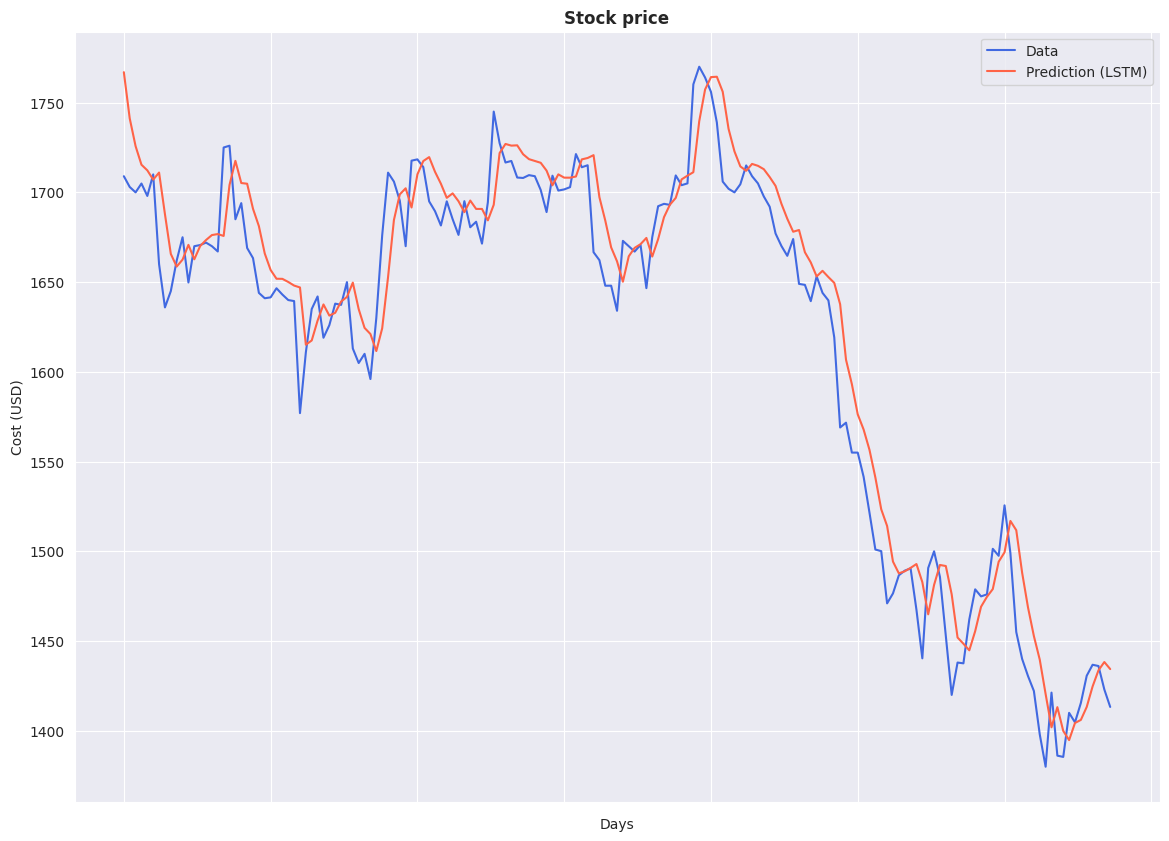
\includegraphics[width=0.8\textwidth]{images/LSTM-600519.png}
        \label{fig:LSTM prediction}
    }
    \hfill
    \subfloat[Transformer]{
        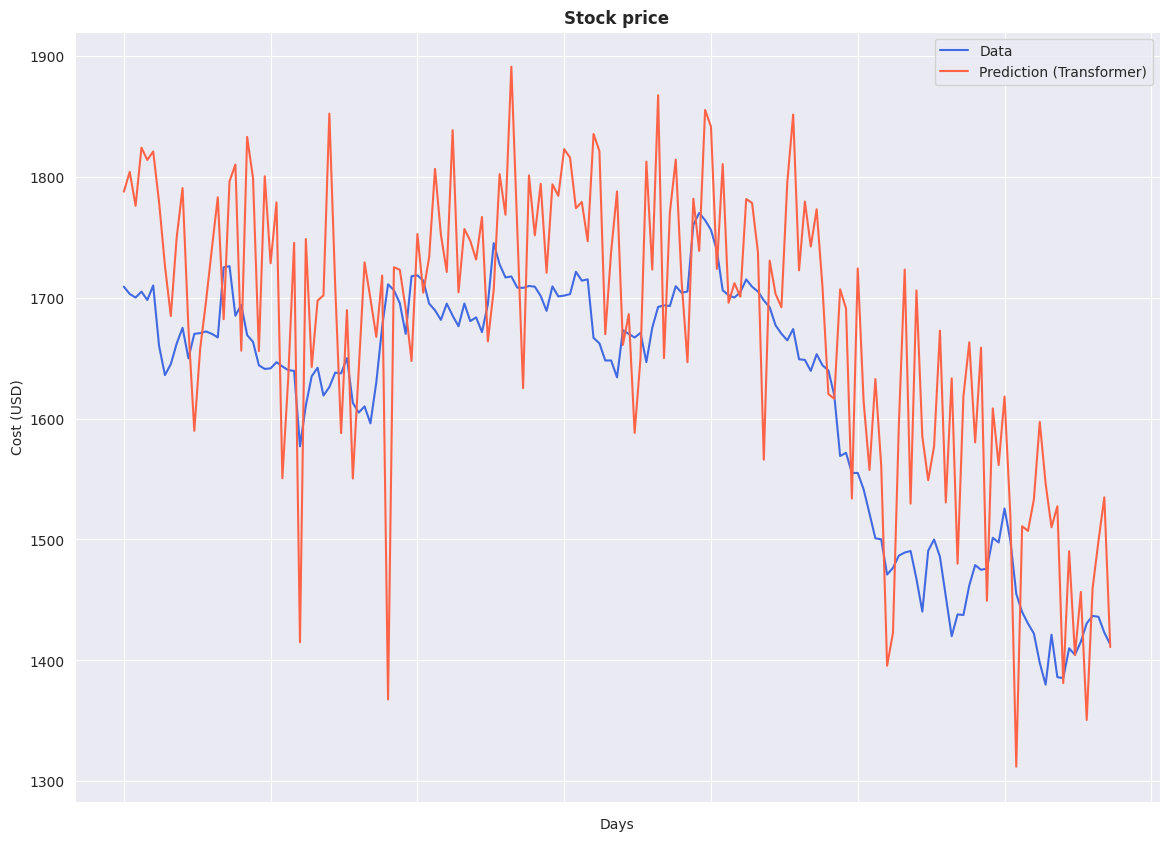
\includegraphics[width=0.8\textwidth]{images/transformer-600519.png}
        \label{fig:transformer prediction}
    }
    \caption{Stock price prediction comparison}
    \label{fig:stock-predict-compare}
\end{figure}

We ran both LSTM, as our base model, and Transformer on a Chinese stock with code $600519$. On the left of Figure \ref{fig:stock-predict-compare}, LSTM is predicted relatively closely and shows a smooth trend. However, on the right, the Transformer's prediction had shown a significant variation with sharp turning points that occurred frequently. Numerically, LSTM's MSE test loss is about $91.84\%$ lower than Transformer's. We reflected on why the prevalent Transformer model failed in such a task. After trying a range of hyperparameters, the Transformer's performance had some minor fluctuation, but the sharp fluctuation remains. By examining the prediction graph of the Transformer, we found out that the general trend for the Transformer is correct. Thus, the high loss is attributed to the sharp peaks and troughs. Conceptually, we guessed it's the attention mechanism that led to this issue. 

\begin{figure}[H]
    \centering
    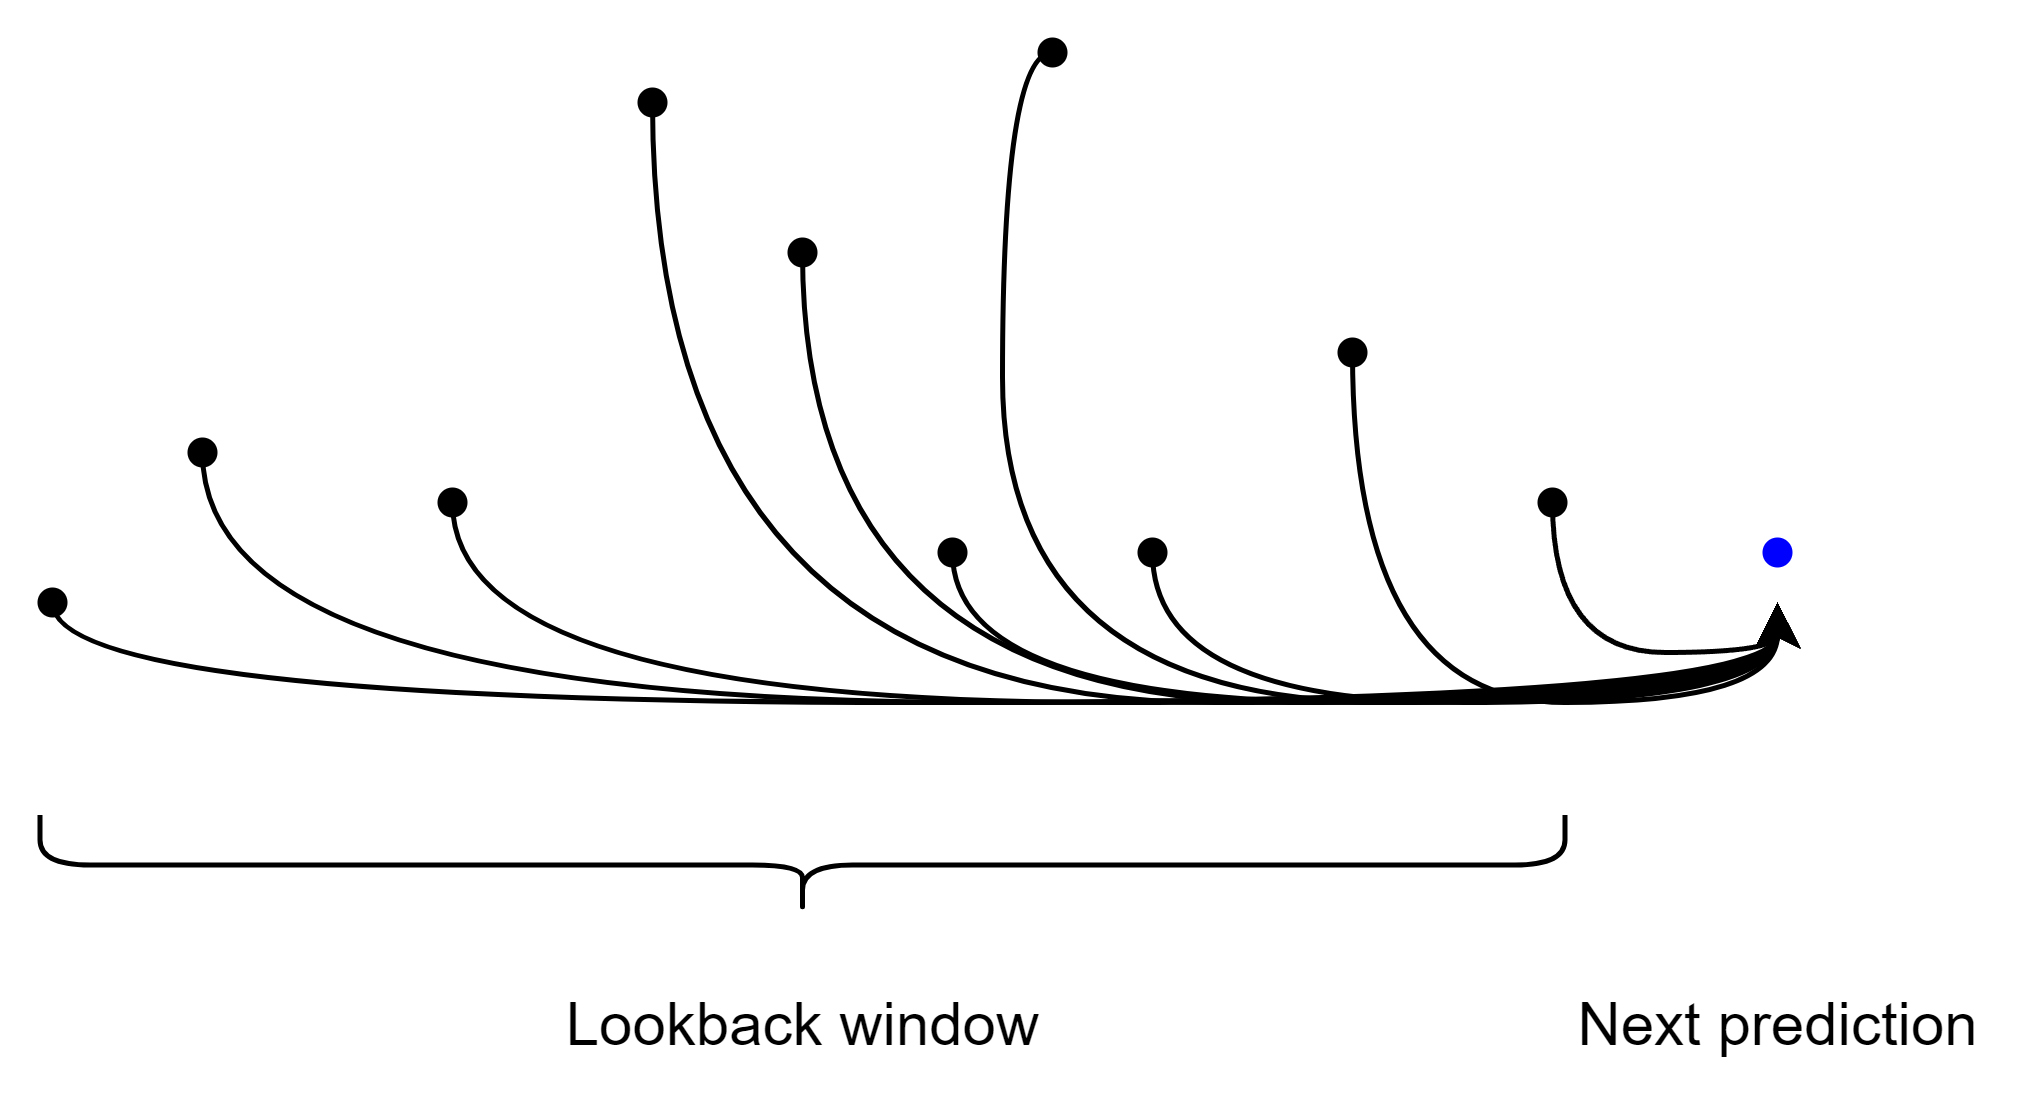
\includegraphics[width=0.8\linewidth]{images/AttentionInTimeSeries.drawio.png}
    \caption{Attention in time series}
    \label{fig:attention-time-series}
\end{figure}

In Figure \ref{fig:attention-time-series}, it illustrates the attention mechanism in time series. Every point in the lookback window (black) will have a weighted contribution to the probability of the next prediction (blue). While this might be successful when the data points are word tokens in Natural Language Processing (NLP), this use of information is too detailed and specific in time series tasks. The model will need to consider every single data point that might fluctuate, leading to increased fluctuation in prediction. As the series increases, there will be more irrelevant fluctuations captured by the Transformer while failing to capture the general trend.  

To address this problem, we used CNN to "summarize" and extract the input features. This can compress a range $k$ data points into a general one, where $k$ is the CNN kernel size while leaving the recent data (last part of data) uncompressed. 

\begin{figure}[H]
    \centering
    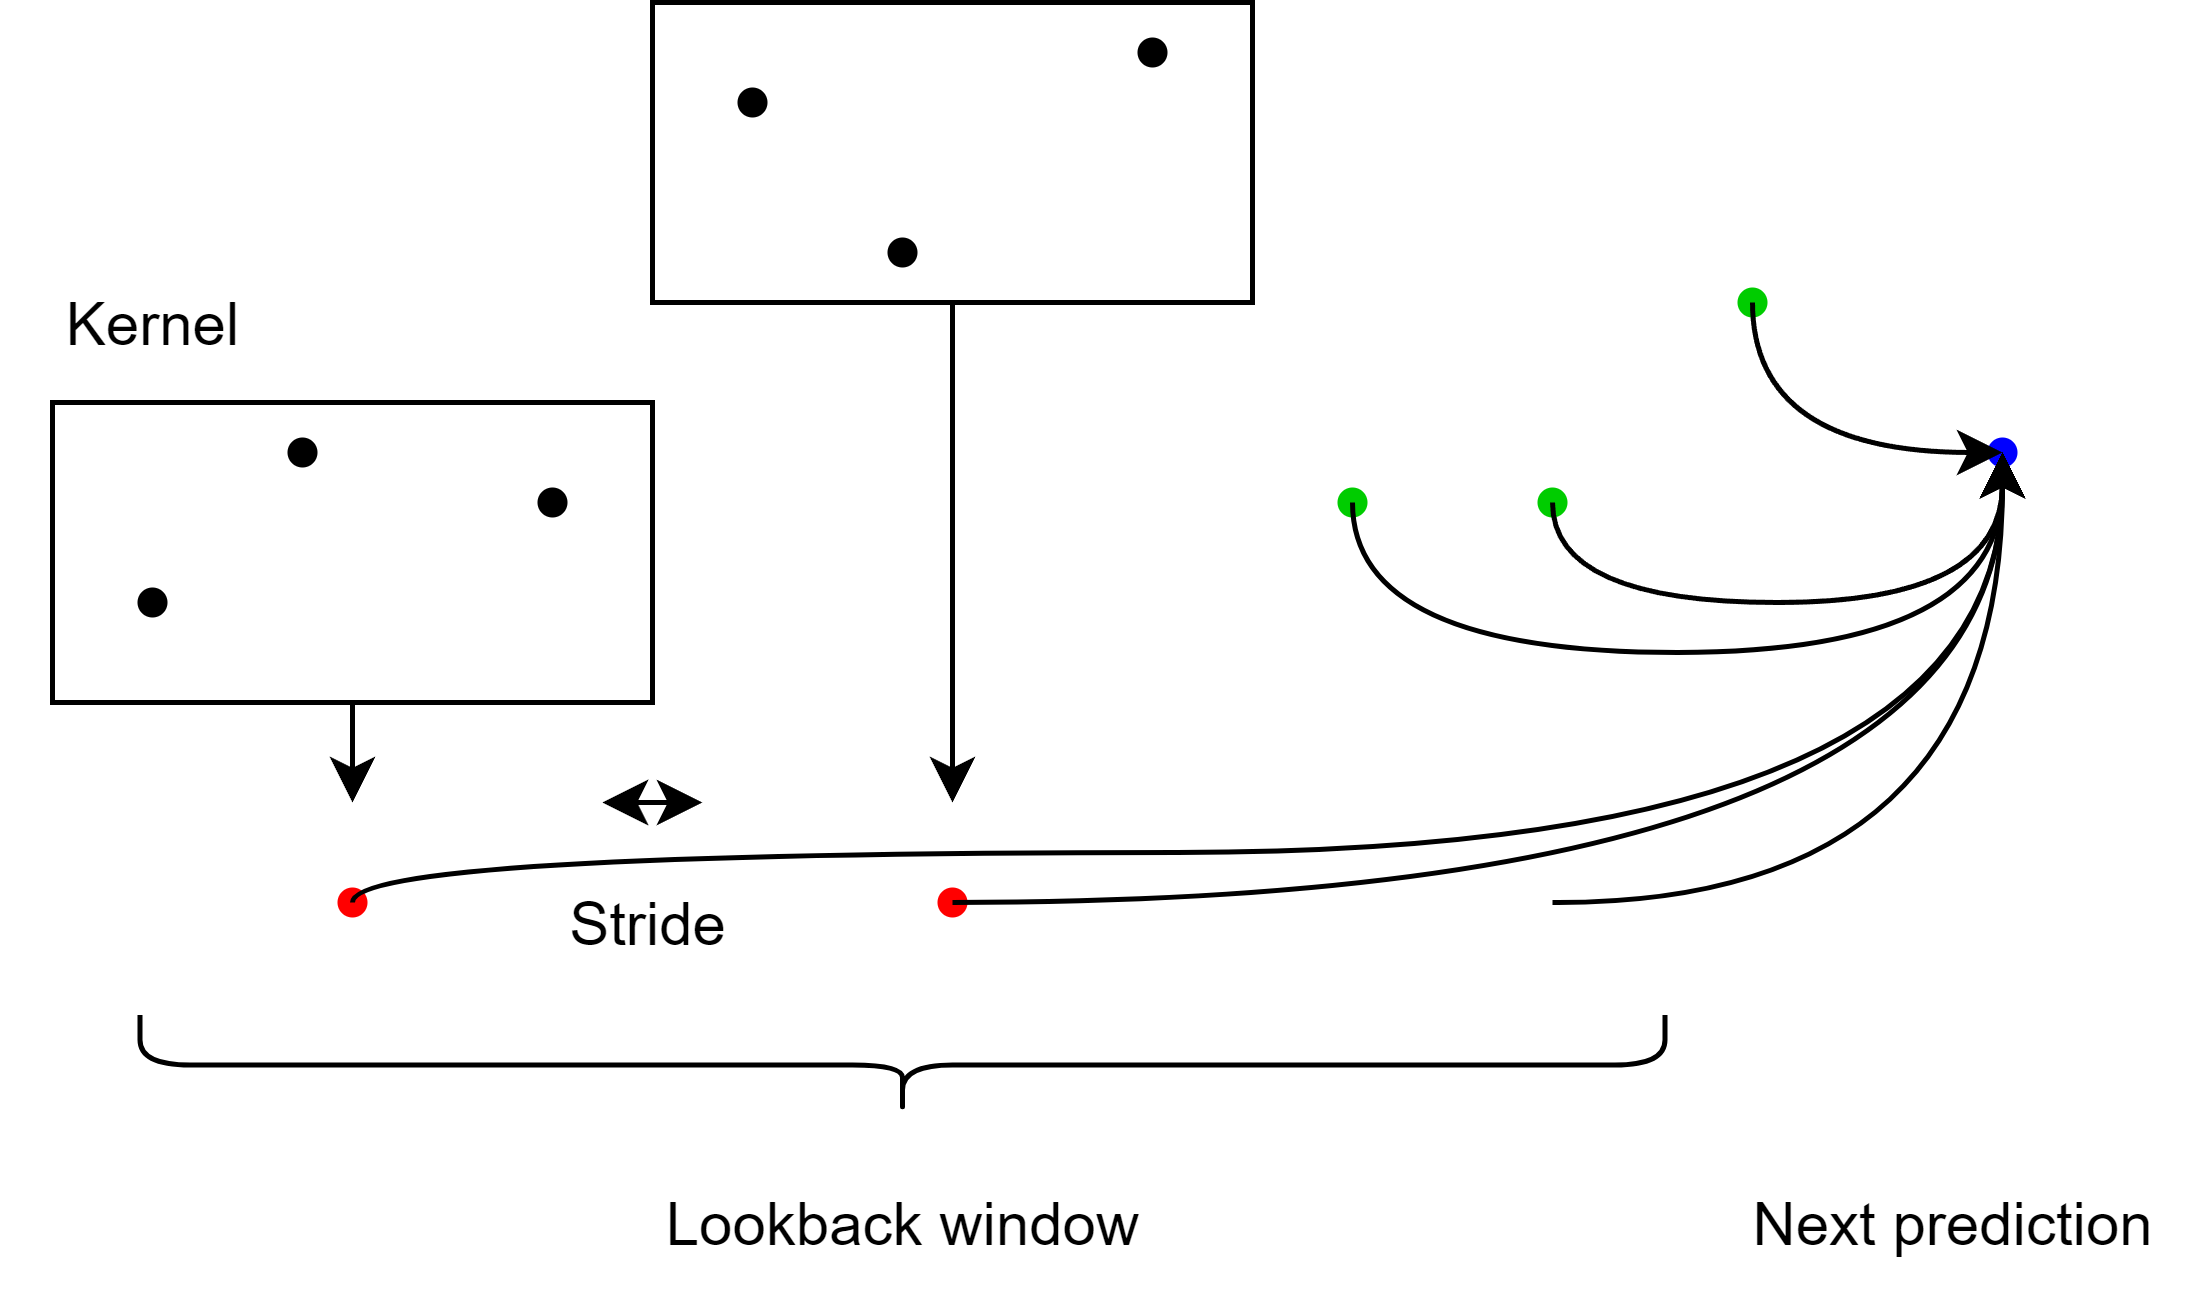
\includegraphics[width=0.8\linewidth]{images/AttentionInTCformer.drawio.png}
    \caption{TCformer attention for time series}
    \label{fig:attention-tcformer}
\end{figure}

In Figure \ref{fig:attention-tcformer}, the kernel of shape 3 is extracting the feature of 3 data points and mapping it into one (red). The distance the kernel moves forward is dependent on the stride. 

The extracted data points (red) along with the raw (green) then applied attention in Transformer. This not only reduces the sequence length but also captures the trend in previous data.

However, this design is based on an important assumption: more recent data in the dataset needs to be more important. This allows us to split the data. This applies to many different datasets, such as traffic, solar, electricity, stock and so on. Conversely, in language models where the input might refer to words in a very early context would not be expected to have an improved precision. 


\section{TCformer}

The architecture we propose is not a specific one but a general idea of how current models can preprocess the input tensor for better efficiency. In this work, we used a simple Encoder for the base model and CNN to preprocess the input. For the most common single-step forecasting task, where the model predicts the next timestamp $X_{n+1}$ by observing the historical data $X_1,..., X_n$.

\subsection{Structure Overview}

\begin{figure}[H]
    \centering
    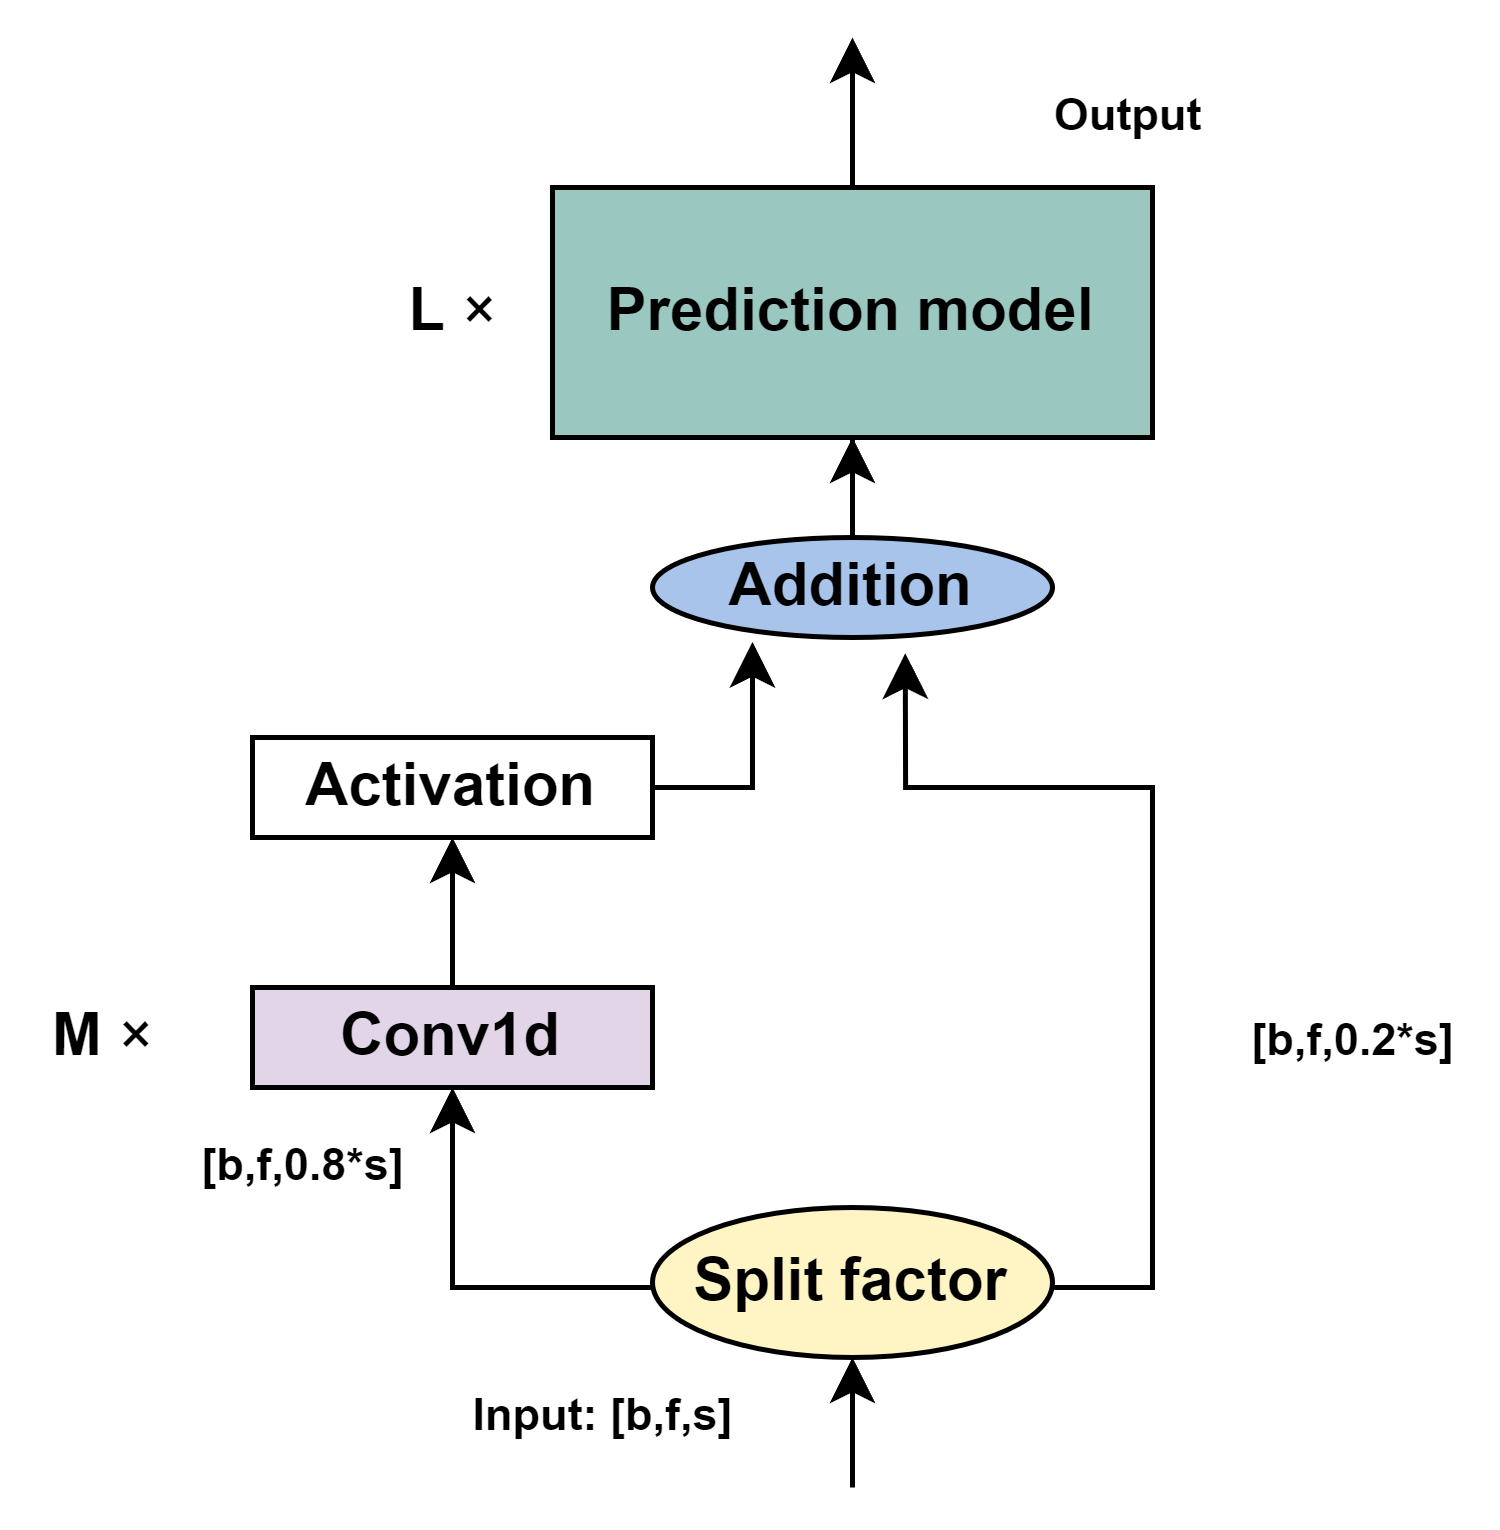
\includegraphics[width=0.8\linewidth]{images/StructureDiagram.drawio.png}
    \caption{TCformer sample structure}
    \label{fig:TCformer-structure}
\end{figure}

The TCformer has a simple and flexible structure. In general, we use CNN for extracting the first $p\%$ of the input data, leaving the rest raw, and feeding it to the prediction model. In Figure \ref{fig:TCformer-structure}, the split factor is a scalar $p$ that splits the dataset into two on the dimension of sequence length. Note that the split factor is a hyperparameter that needs to be manually assigned. For example, a scalar $p=0.8$ would split the input of shape $X\in \mathbb{R}^{b,f,s}$ into $X\in \mathbb{R}^{b,f,0.8\cdot s}$ and $X\in \mathbb{R}^{b,f,0.2\cdot s}$ where:

\begin{enumerate}
    \item $b$ is the batch size
    \item $f$ is the dimension of the feature
    \item $s$ is the sequence length
\end{enumerate}

In Figure \ref{fig:TCformer-structure}, there can be $M$ Conv1d layer. They are 1-dimensional convolution layers that extract traits from the $p\%$ of the input and reduce the sequence length, where $p$ is the split factor and it's set to $0.8$ in this illustration. There could be multiple layers added flexibly. It can be replaced by a Conv2d (needs to ensure that the dimension of the model doesn't reduce). The right branch leaves the raw data that will be joined back with the left branch in the concat component. In the concatenated component, the two branches' tensors will be merged on the third dimension $s$. Lastly, the concatenated tensor will be the input for the prediction model. 

\subsection{Convolution extraction}

\begin{figure}[H]
    \centering
    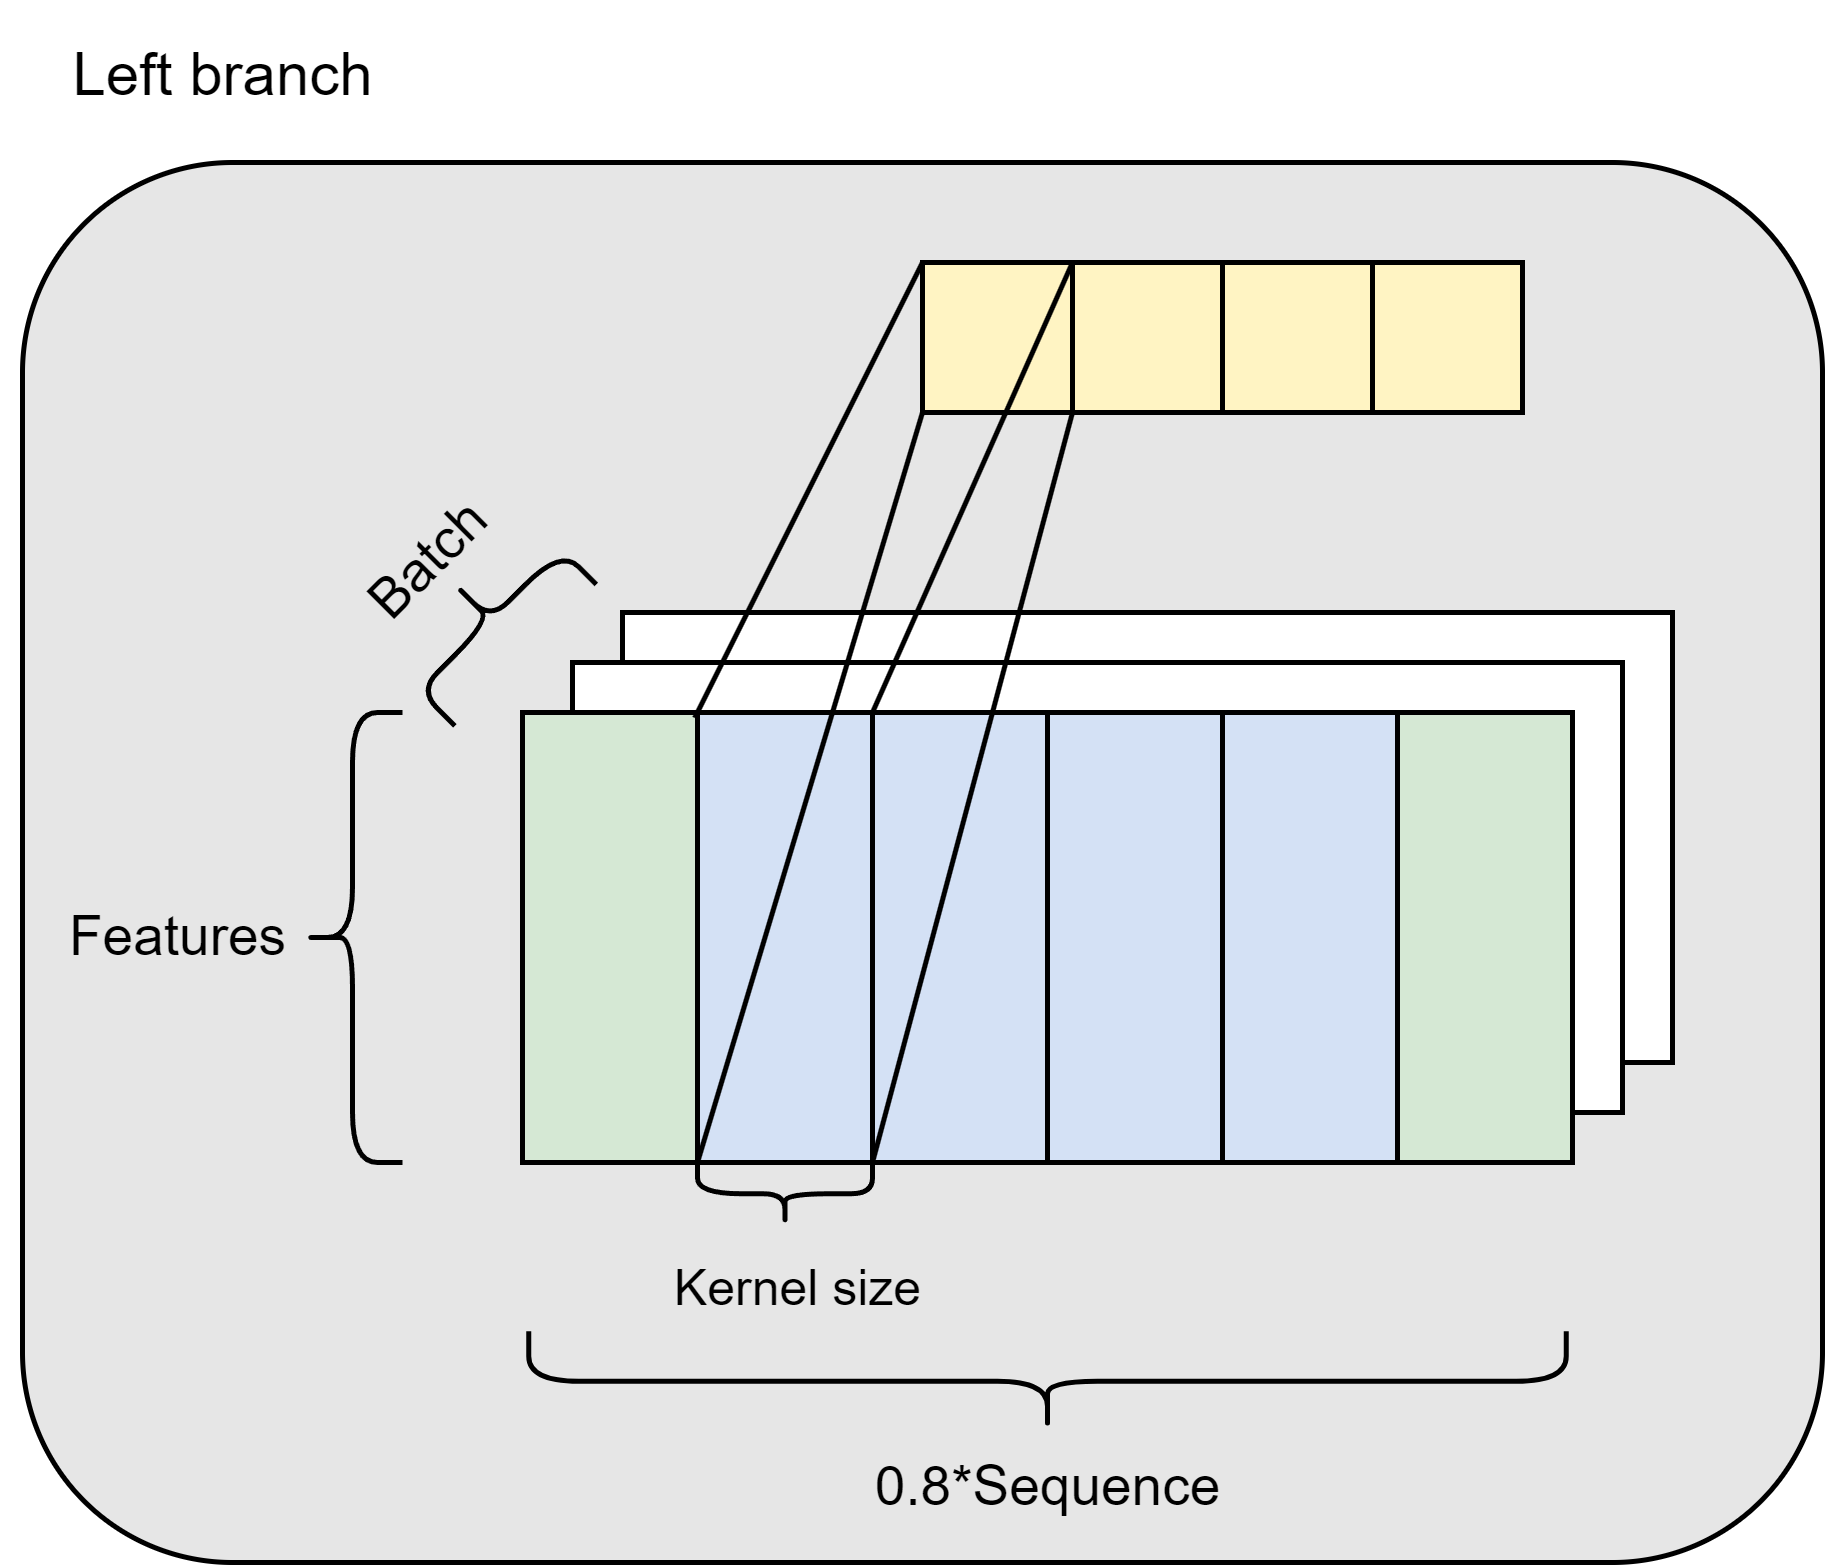
\includegraphics[width=0.7\linewidth]{images/Left branch.png}
    \caption{Convolutional sequence summary on left branch}
    \label{fig:convolutional-operation}
\end{figure}

In the left branch illustrated in \ref{fig:convolutional-operation}, the Conv1d layer is outputting summaries for the first $80\%$ of earlier data, leaving the rest $20\%$ raw for the Transformer encoder to process. This will cause the input $X$ to change its third dimension's shape $s$ from:

\begin{gather}
    s_1=0.8\cdot s\\
    s_2=\lfloor\frac{0.8\cdot s-k}{r} \rfloor+1
\end{gather}

\begin{enumerate}
    \item $s_1$ is the sequence length before the convolution layer
    \item $k$ is kernel size
    \item $s_2$ is the sequence length after the convolution layer
    \item $r$ is the stride
\end{enumerate}

On the right branch, the raw data is not processed. Given that the Transformer has already a good performance on raw data, applying convolution is not needed and might reduce the information perceived in the encoder block. 

\subsection{Sequence length reduction}
\label{sec:seq-len-reduction}

After the addition, the input for the encoder block will have a sequence length of:

\begin{gather}
    s_3=s_2+0.2\cdot s\\
    =\lfloor\frac{0.8\cdot s-k}{r} \rfloor+1+0.2\cdot s
\end{gather}

The reduction of sequence length $s_3$ compared to $s$ can be calculated:

\begin{gather}
    l=s-s_3\\
    =s-\lfloor\frac{0.8\cdot s-k}{r} \rfloor-1-0.2\cdot s
\end{gather}

Notice $l$ is positively related with $k$ and $r$, changing the stride and kernel size can give a flexible control on the model size. In the attention block, a reduction of $l$ will reduce:

\begin{gather}
    l\times b\times f
\end{gather}

in each of the $Q,K,V$ matrices, largely reducing its parameters.

\section{Experiments}
We experimented with the model on both single-step prediction and sequence-to-sequence (seq2seq) tasks. 

\subsection{Experiments for single-step prediction}

We conducted experiments on 3 real-world datasets in the experiment, including weather used in Autoformer \cite{autoformer} and AMD stock data. 

\subsubsection{Dataset}

The weather dataset included 52696 rows of data with 21 covariates. 

The AMD stock dataset is accessed through Baostock API \cite{baostock}. It includes 10995 rows of data with 5 covariates. The data spans from the 2nd of January 1981 to the 14th of August 2024. 

\subsubsection{Experiment setup}

The transformer model has a hidden dimension of 8, 2 layers, and 2 heads for attention. For all models, the optimizer uses Adam, with lr=1e-3, wd=1e-4, dropout=0.1, training in 5 epochs with a batch size of 512 with train test $9:1$ splitting. The TCformer uses a split factor of 0.8 with the CNN using kernel size 6 with a stride of 6. The criteria uses MSE (Mean Squared Error). 

\subsubsection{Results}

\begin{table}[H]
\centering
\begin{tabular}{rrrr}
\toprule
TCformer1d & transformer & seq\_len & pct\_improve(\%) \\
\midrule
0.018490 & 0.073744 & 16 & 74.93 \\
0.015125 & 0.061805 & 32 & 75.53 \\
0.012830 & 0.053022 & 64 & 75.80 \\
0.017049 & 0.069303 & 128 & 75.40 \\
0.016919 & 0.070958 & 256 & 76.16 \\
0.017332 & 0.072824 & 512 & 76.20 \\
\bottomrule \\
\end{tabular}
\caption{AMD stock data test MSE loss}
\label{tab:AMD-loss}
\end{table}

In Table \ref{tab:AMD-loss}, for AMD stock data, the TCformer with 1d on average has improved performance by about 75\% while having reduced size of the model. During the experiment, the TCformer was successfully trained on the dataset when the sequence length is 1024 however the Transformer model failed due to GPU memory overflow, so the sequence length for the experiment is limited up to $512$.

\begin{figure}[H]
    \centering
    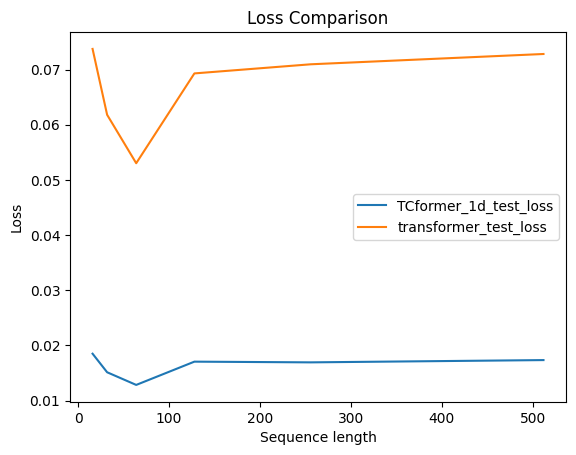
\includegraphics[width=0.8\linewidth]{images/AMD-loss-cmp.png}
    \caption{AMD loss curve}
    \label{fig:AMD-loss-curve}
\end{figure}

In Figure \ref{fig:AMD-loss-curve}, the test loss for both models has it's minimum at a sequence length of 64. For every sequence length, the TCformer has a much lower loss compared to Transformer. The Transformer loss shows an increase as sequence length increases from 128 to 512 while this is relatively not as significant in TCformer's loss. This shows that the sequence reduction has enabled TCformer to handle longer sequences while maintaining similar precision. 

\begin{table}[H]
\centering
\begin{tabular}{rrrr}
\toprule
TCformer1d & transformer & seq\_len & pct\_improve (\%) \\
\midrule
0.026144 & 0.104435 & 16 & 74.97 \\
0.026144 & 0.104253 & 32 & 74.92 \\
0.026188 & 0.103928 & 64 & 74.80 \\
0.025542 & 0.101652 & 128 & 74.87 \\
0.028019 & 0.107837 & 256 & 74.02 \\
0.026371 & 0.104923 & 512 & 74.87 \\
\bottomrule\\
\end{tabular}
\caption{Weather data test MSE loss}
\label{tab:weather-loss}
\end{table}

Like the results in Table \ref{tab:AMD-loss}, the percentage improved is around $74\%$ in Table \ref{tab:weather-loss}. Given that Transformer has a poor performance, this great improvement is within expectation. 


\begin{figure}[H]
    \centering
    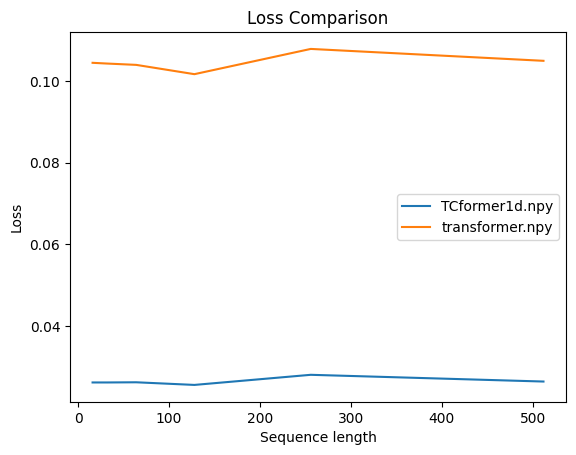
\includegraphics[width=0.8\linewidth]{images/weather-loss-cmp.png}
    \caption{Weather loss curve}
    \label{fig:weather-loss-curve}
\end{figure}

\subsection{Experiments for sequence to sequence}

\subsubsection{Dataset}

For sequence to sequence, we used 7 datasets (ECL, ETT subset 1, Exchange, Traffic, Weather, and Solar energy), the same as the experiment for iTransformer \cite{liu2023itransformer}. For each dataset, we ran Transformer, iTransformer, and TCiTransformer (iTransformer with CNN). Since iTransformer currently has the best accuracy on different datasets, we used it as our prediction model, simply replacing the TCformer's Transformer Encoder with the iTransformer Encoder. 

The dataset covers a range of samples and feature sizes:

\begin{figure}[H]
    \centering
    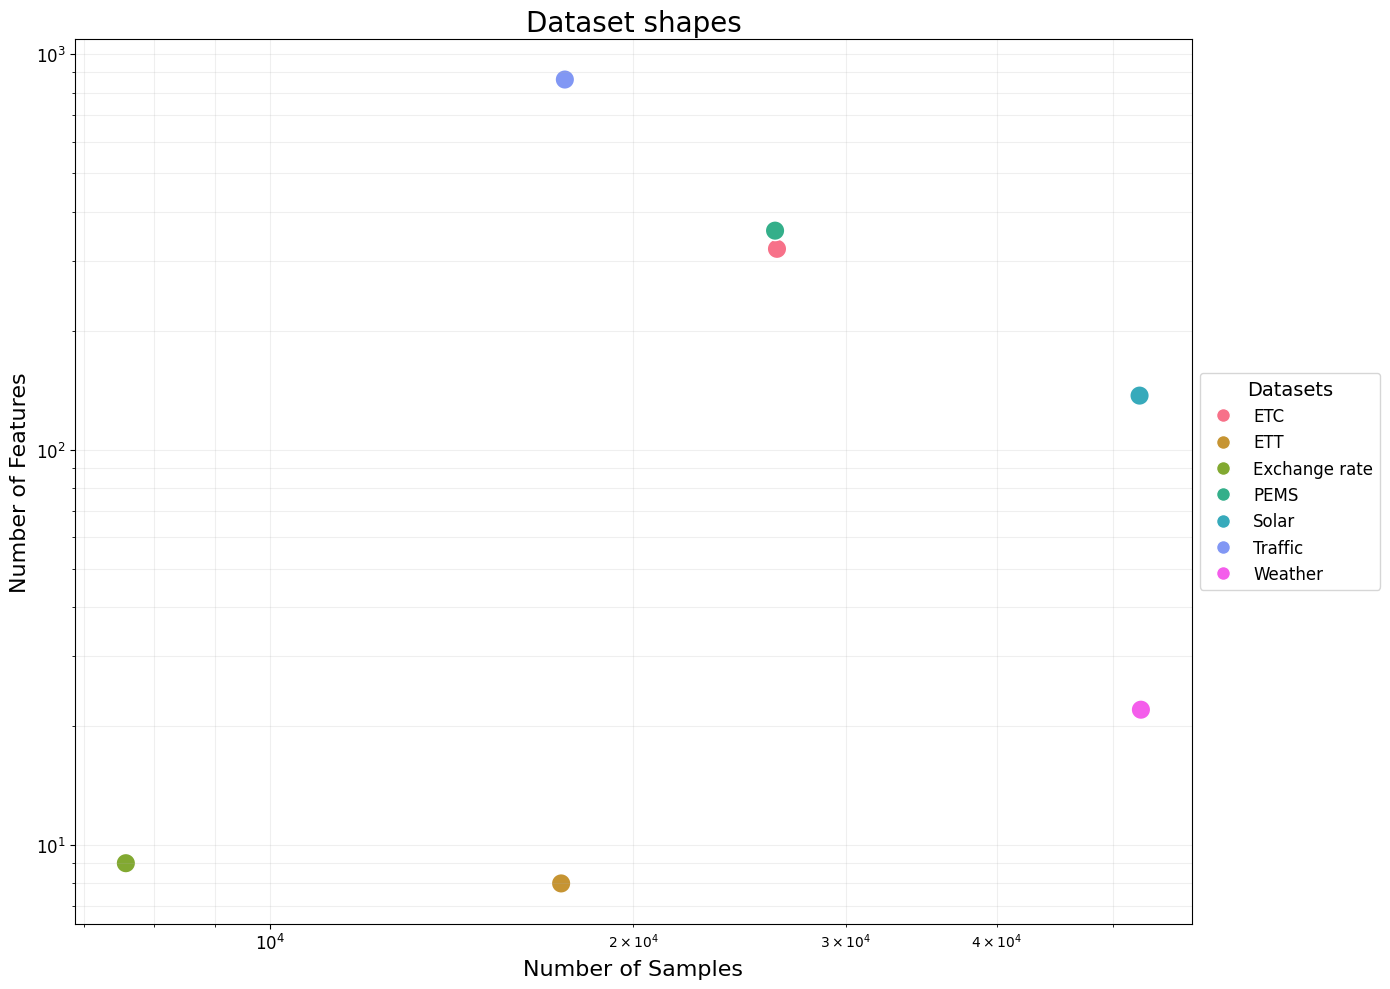
\includegraphics[width=0.8\linewidth]{images/dataset-shape.png}
    \caption{Dataset shapes}
    \label{fig:dataset-shape}
\end{figure}

\subsubsection{Experiment setup}
For each model, we set the prediction length to \(P=\{96,192,336\}\) and the lookback length to 96. Since PEMS is too large, we set the lookback 48 and prediction length to \(P=\{12,24,48\}\). We set two layers of CNN, and split factor to 0.8 for the iTransformer with CNN. The kernel of the first layer is 5, stride 2 and the second layer is 3, stride 1. We experimented with the model with different hyperparameters such as the CNN kernel size, stride, split factors and so on. The impact on the performance isn't obvious, so we set two layers to have the kernel capturing 9 timestamps at each time. This ensures that most of the dataset doesn't cover a whole period but extracts the trends that exist in a period and then gives it to the prediction model. The kernel isn't set too small to ensure that it can reduce the sequence length.

\subsubsection{Results}
\label{sec:seq2seq-result}

\begin{table}[H]
    \centering
    \begin{tabular}{llrrrr}
    \hline
    Dataset & Model & MSE & MAE & Input\ length & Output\ length \\
    \hline
    ECL & Transformer & 0.249665 & 0.349949 & 96 & 96 \\
    ECL & iTransformer & 0.167462 & 0.256914 & 96 & 96 \\
    ECL & TCiTransformer & 0.180147 & 0.280937 & 96 & 96 \\
    ETTh1 & Transformer & 0.796016 & 0.702380 & 96 & 96 \\
    ETTh1 & iTransformer & 0.387790 & 0.406386 & 96 & 96 \\
    ETTh1 & TCiTransformer & 0.393983 & 0.415327 & 96 & 96 \\
    Exchange & Transformer & 0.677474 & 0.637843 & 96 & 96 \\
    Exchange & iTransformer & 0.086314 & 0.206543 & 96 & 96 \\
    Exchange & TCiTransformer & 0.086183 & 0.207386 & 96 & 96 \\
    PEMS03 & Transformer & 0.105133 & 0.204023 & 48 & 12 \\
    PEMS03 & iTransformer & 0.073994 & 0.179749 & 48 & 12 \\
    PEMS03 & TCiTransformer & 0.066601 & 0.170845 & 48 & 12 \\
    solar & Transformer & 0.198320 & 0.232168 & 96 & 192 \\
    solar & iTransformer & 0.212609 & 0.245238 & 96 & 96 \\
    solar & TCiTransformer & 0.224425 & 0.245268 & 96 & 96 \\
    traffic & Transformer & 0.665396 & 0.365834 & 96 & 96 \\
    traffic & iTransformer & 0.465135 & 0.323030 & 96 & 96 \\
    traffic & TCiTransformer & 0.546155 & 0.343953 & 96 & 192 \\
    weather & Transformer & 0.221558 & 0.310034 & 96 & 96 \\
    weather & iTransformer & 0.183019 & 0.224638 & 96 & 96 \\
    weather & TCiTransformer & 0.167566 & 0.213238 & 96 & 96 \\
    \hline\\
    \end{tabular}
    \caption{Summary table for loss (selecting lowest MSE)}
    \label{tab:summary-table}
\end{table}

For each model on each dataset, we selected it's the best-performing results from the varying output sequence length. In Table \ref{tab:summary-table}, iTransformer1dSplit is the iTransformer with CNN. For the seq2seq task, the TCiTransformer didn't have much increase compared to iTransformer in most datasets. In ECL, ETTh1, solar and traffic, the model's precision is lower than iTransformer. However, in PEMS03, Exchange and weather, TCiTransformer had a higher precision. The full result is in Appendix \ref{sec:full-result}.

\begin{figure}[H]
    \centering
    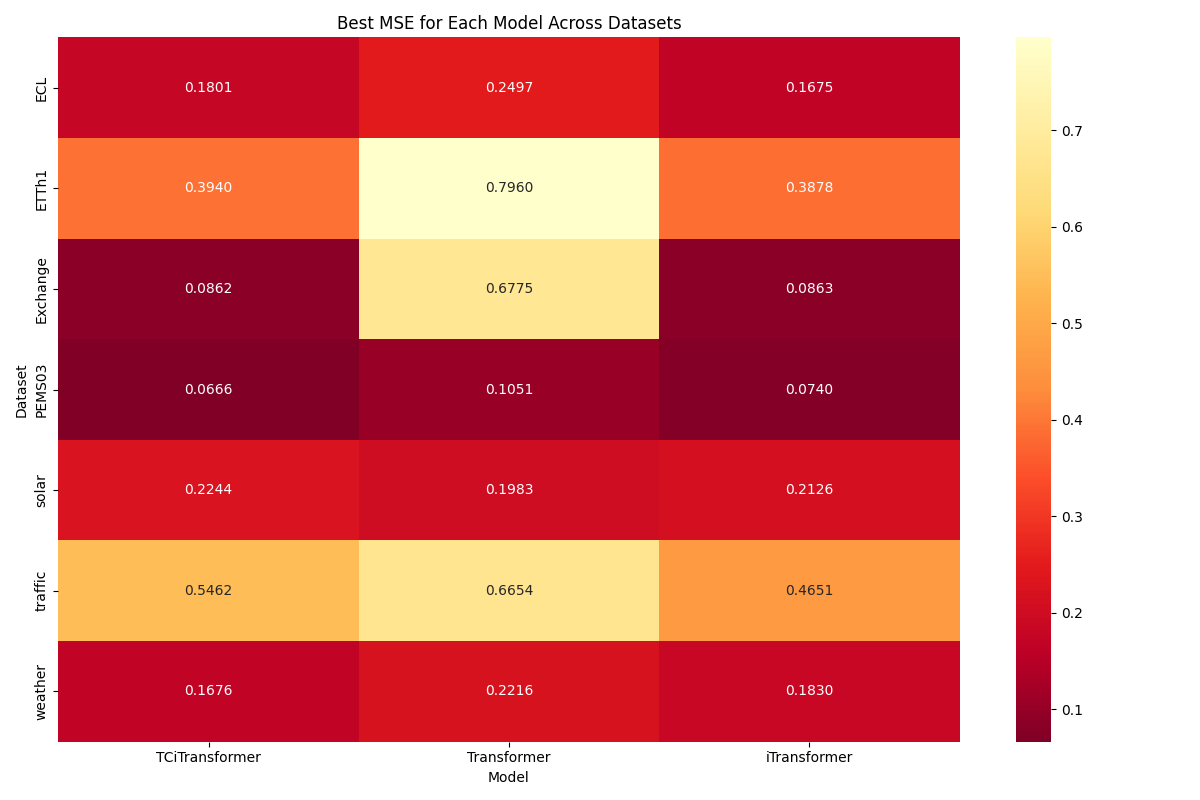
\includegraphics[width=\linewidth]{images/mse_heatmap.png}
    \caption{MSE heatmap}
    \label{fig:mse-heatmap}
\end{figure}

This is illustrated clearer in Figure \ref{fig:mse-heatmap}. The darker means the better the model is.

We selected the prediction of our model on traffic, which it's performing worse, and weather which it performs better:

\begin{figure}[H]
    \centering
    \subfloat[traffic]{
        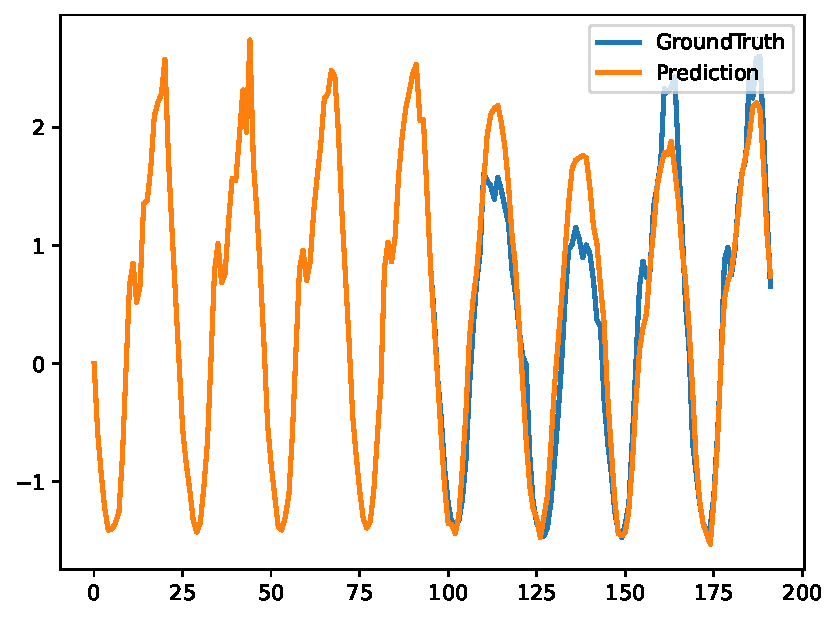
\includegraphics[width=0.45\textwidth]{images/traffic-TCiTrans.pdf}
        \label{fig:traffic-pred}
    }
    \hfill
    \subfloat[weather]{
        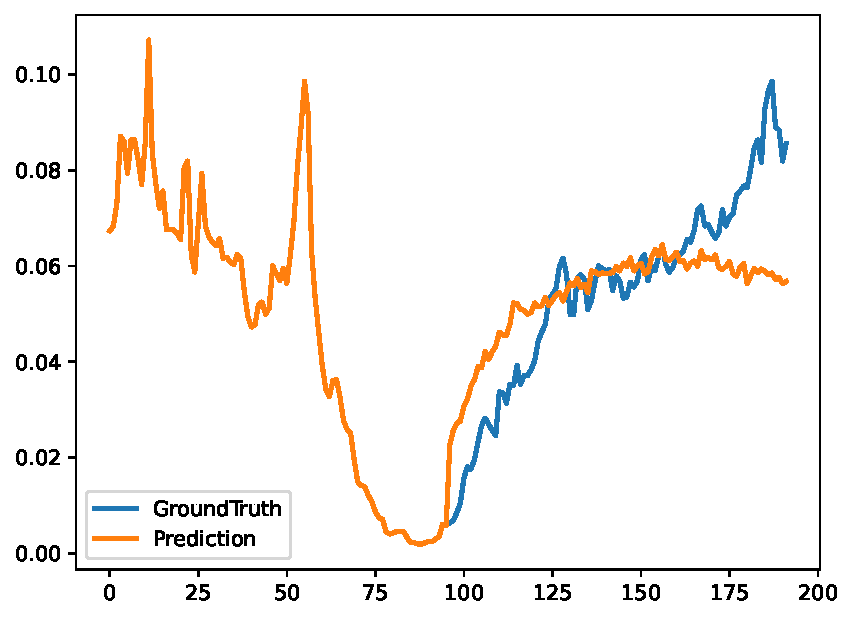
\includegraphics[width=0.45\textwidth]{images/weather-TCiTrans.pdf}
        \label{fig:weather-pred}
    }
    \caption{Prediction on traffic and Weather for both input and output length is 96}
    \label{fig:TCiTrans-compare}
\end{figure}

The traffic data is much more periodic with a generally regular pattern, while the weather data is more irregular. By observing other datasets, we found out that TCiTransformer is better in non-periodic time series forecasting. This might be because the CNN cannot be trained to capture the increase and decrease over a small range of time, while it gives the general trend in datasets such as weather.

\subsubsection{Efficiency}
Although the sequence length can be reduced, as mentioned in section \ref{sec:seq-len-reduction}, the CNN requires time for operation. Depending on the kernel size and stride, the time for TCformer architecture can vary. In the experiments above, we recorded the training time for traffic data, using the same kernel size and stride: 

\begin{figure}[H]
    \centering
    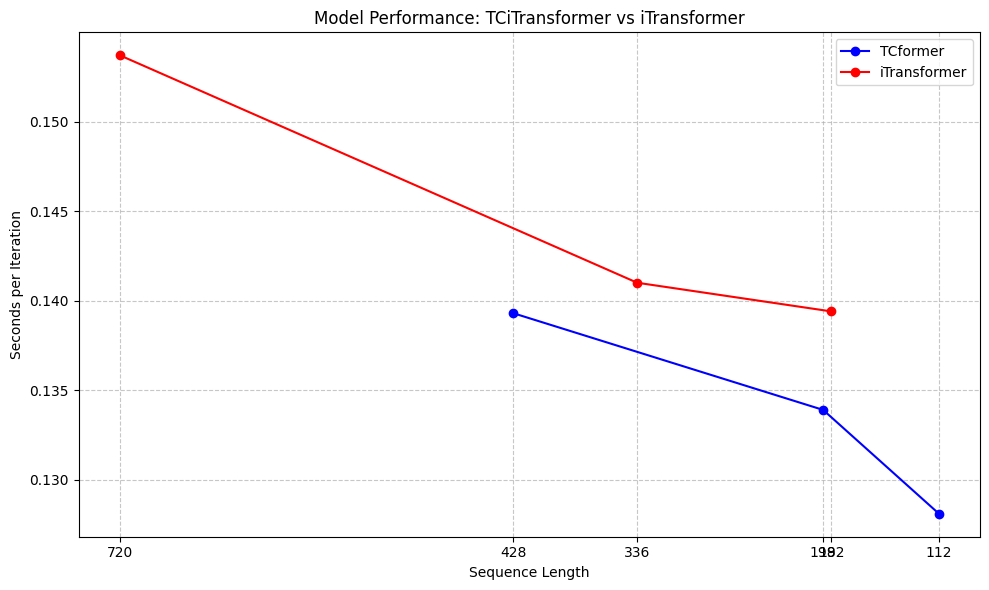
\includegraphics[width=0.8\linewidth]{images/efficiency-cmp1.png}
    \caption{Speed comparison on different sequence length scale}
    \label{fig:efficiency-cmp1}
\end{figure}

Fig.\ref{fig:efficiency-cmp1} shows the speed of TCiTransformer against iTransformer. Because TCformer architecture reduces the sequence length, so there is a right shift of the blue line on the sequence length. However, even at the same sequence length, TCiTransformer outperformed iTransformer.

\begin{figure}[H]
    \centering
    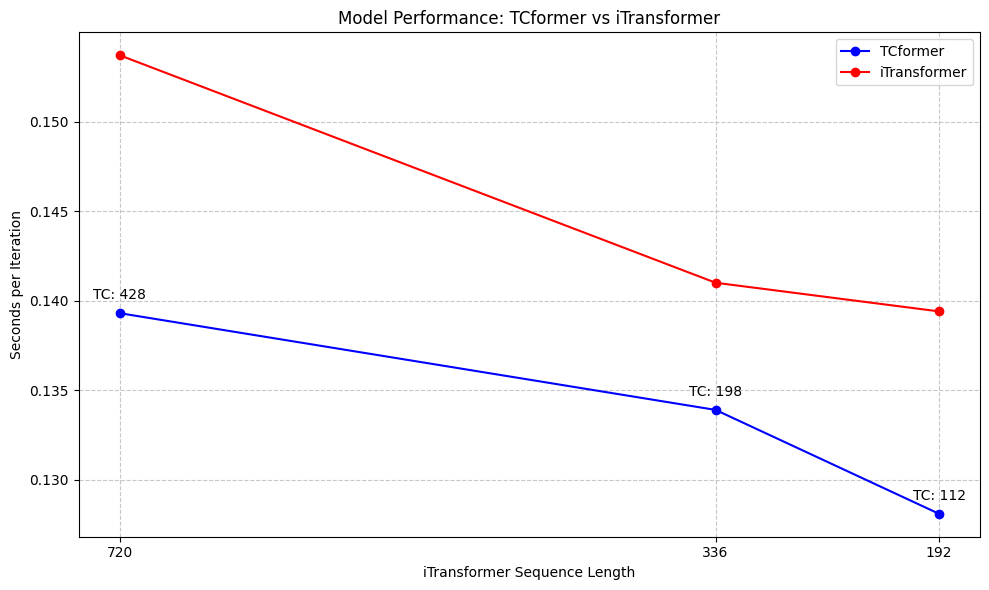
\includegraphics[width=0.8\linewidth]{images/efficiency-cmp2.png}
    \caption{Speed comparison on same sequence length scale}
    \label{fig:efficiency-cmp2}
\end{figure}

Fig.\ref{fig:efficiency-cmp2} plots the speed of the model on the same sequence length scale. It shows at the same input sequence length, the reduced encoder block input will lead to an increase in speed, despite the cost of CNN calculation. 

These results show that the CNN layers in TCformer does lead to an improvement in efficiency.


\section{Conclusion and Evaluation}

Overall, the TCformer architecture is successful in addressing the limitations of both pure convolutional and transformer models. By integrating temporal convolution with transformer-based attention, TCformer achieves superior predictive performance in single-step prediction tasks while maintaining computational efficiency. The model's ability to handle longer sequences and its consistent performance improvements across different datasets suggest its potential for wide applicability in various time series prediction tasks. As datasets continue to grow in size and complexity, current models need to increase their model dimensions to handle longer sequence lengths. However, with TCformer, the prediction model receives a reduced sequence length. Lastly, the model offers flexibility in determining the split factor, layers of CNN and the prediction model, allowing researchers to use this general architecture in various forms. 

The performance improvement, in general, didn't exist in seq2seq task. The mediocre performance suggests that using CNN to extract features might not help predict periodic datasets, as mentioned previously. However, TCformer could still be applied for improving efficiency.

\section{Future works}

Because TCformer is an architectural change, rather than a change in components, it's compatible with the whole family of Transformer models, such as Autoformer \cite{autoformer}, informer \cite{informer} and so on. Future works can be done to investigate TCformer's impact on these models. Not only transformers but other families of models such as RNN, LSTM, and Mamba \cite{mamba2} can incorporate this idea for data processing. 

In this work, we applied 1D CNN layers for feature extraction. 2D CNN layers could be used in substitution to allow blocks of data, like patches in PatchTST \cite{nie2023timeseriesworth64} and extract the input data across different features. 

We believe this idea of "compressing" the inputs partially can become a generalized approach in time series tasks for better model efficiency while improving or maintaining precision. There could be other better approaches to "compress" the data partially, other than CNN, to improve the performance and efficiency of current models. 

Since TCformer had a great result in single-step prediction tasks, changing the encoder-only architecture of iTransformer and using decoders to make the model autoregressive might bring improved performance for TCformer in seq2seq tasks. 

Moreover, Kolomogorov-Arnold Networks (KAN) can be more expressive in each neuron, so using it in the TCformer feed-forward network might be also a way to reduce the parameters \cite{kan}. 

Rather than changing the architecture, future works can also explore how to utilize the idea at the component level, such as incorporating it into the attention mechanism. 

\printbibliography

\appendix
\label{sec:full-result}
\section{Full result}
The full result of seq2seq task:

    
\begin{longtable}{llrrrr}
\caption{Performance comparison of different models across various datasets}\label{tab:long_performance} \\

\toprule
Dataset & Model & Input\_length & Output\_length & MSE & MAE \\
\midrule
\endfirsthead

\multicolumn{6}{c}%
{\tablename\ \thetable\ -- \textit{Continued from previous page}} \\
\toprule
Dataset & Model & Input\_length & Output\_length & MSE & MAE \\
\midrule
\endhead

\midrule
\multicolumn{6}{r}{\textit{Continued on next page}} \\
\endfoot

\bottomrule
\endlastfoot
ECL &         Transformer &            96 &             96 & 0.311263 & 0.398829 \\
         ECL &         Transformer &            96 &            192 & 0.344802 & 0.426795 \\
         ECL &         Transformer &            96 &            336 & 0.348473 & 0.427140 \\
         ECL &         Transformer &           192 &            336 & 0.356725 & 0.433641 \\
         ECL &         Transformer &           336 &            336 & 0.354477 & 0.429831 \\
         ECL &         Transformer &           720 &            336 & 0.360726 & 0.429443 \\
         ECL &        iTransformer &            96 &             96 & 0.189476 & 0.275656 \\
         ECL &        iTransformer &            96 &            192 & 0.200119 & 0.287542 \\
         ECL &        iTransformer &            96 &            336 & 0.220469 & 0.307598 \\
         ECL &        iTransformer &           192 &            336 & 0.191621 & 0.291078 \\
         ECL &        iTransformer &           336 &            336 & 0.190013 & 0.282944 \\
         ECL &        iTransformer &           720 &            336 & 0.209483 & 0.307388 \\
         ECL & iTransformer1dSplit &            96 &             96 & 0.195807 & 0.295794 \\
         ECL & iTransformer1dSplit &            96 &            192 & 0.209703 & 0.306293 \\
         ECL & iTransformer1dSplit &            96 &            336 & 0.229005 & 0.324030 \\
         ECL & iTransformer1dSplit &           192 &            336 & 0.209419 & 0.312572 \\
         ECL & iTransformer1dSplit &           336 &            336 & 0.218014 & 0.321793 \\
         ECL & iTransformer1dSplit &           720 &            336 & 0.214763 & 0.322888 \\
       ETTh1 &         Transformer &            96 &             96 & 0.903719 & 0.770211 \\
       ETTh1 &         Transformer &            96 &            192 & 0.892692 & 0.757590 \\
       ETTh1 &         Transformer &            96 &            336 & 0.982860 & 0.801562 \\
       ETTh1 &        iTransformer &            96 &             96 & 0.389884 & 0.406386 \\
       ETTh1 &        iTransformer &            96 &            192 & 0.446103 & 0.440019 \\
       ETTh1 &        iTransformer &            96 &            336 & 0.487570 & 0.462899 \\
       ETTh1 & iTransformer1dSplit &            96 &             96 & 0.393983 & 0.415327 \\
       ETTh1 & iTransformer1dSplit &            96 &            192 & 0.446689 & 0.444733 \\
       ETTh1 & iTransformer1dSplit &            96 &            336 & 0.488159 & 0.467200 \\
    Exchange &         Transformer &            96 &             96 & 0.677474 & 0.665115 \\
    Exchange &         Transformer &            96 &            192 & 1.226818 & 0.894968 \\
    Exchange &         Transformer &            96 &            336 & 1.227765 & 0.949669 \\
    Exchange &        iTransformer &            96 &             96 & 0.086843 & 0.206637 \\
    Exchange &        iTransformer &            96 &            192 & 0.182796 & 0.305740 \\
    Exchange &        iTransformer &            96 &            336 & 0.334583 & 0.420060 \\
    Exchange & iTransformer1dSplit &            96 &             96 & 0.086183 & 0.207386 \\
    Exchange & iTransformer1dSplit &            96 &            192 & 0.177637 & 0.300582 \\
    Exchange & iTransformer1dSplit &            96 &            336 & 0.364597 & 0.432012 \\
      PEMS03 &         Transformer &            48 &             12 & 0.116023 & 0.216098 \\
      PEMS03 &         Transformer &            48 &             24 & 0.134372 & 0.237528 \\
      PEMS03 &         Transformer &            48 &             48 & 0.141914 & 0.245927 \\
      PEMS03 &        iTransformer &            48 &             12 & 0.074810 & 0.181082 \\
      PEMS03 &        iTransformer &            48 &             24 & 0.115063 & 0.225679 \\
      PEMS03 &        iTransformer &            48 &             48 & 0.211413 & 0.308824 \\
      PEMS03 & iTransformer1dSplit &            48 &             12 & 0.066601 & 0.170845 \\
      PEMS03 & iTransformer1dSplit &            48 &             24 & 0.738303 & 0.668719 \\
      PEMS03 & iTransformer1dSplit &            48 &             48 & 1.097343 & 0.826441 \\
       solar &         Transformer &            96 &             96 & 0.217859 & 0.232168 \\
       solar &         Transformer &            96 &            192 & 0.198320 & 0.241451 \\
       solar &         Transformer &            96 &            336 & 0.216907 & 0.252444 \\
       solar &        iTransformer &            96 &             96 & 0.213345 & 0.254571 \\
       solar &        iTransformer &            96 &            192 & 0.247524 & 0.283152 \\
       solar &        iTransformer &            96 &            336 & 0.263141 & 0.294588 \\
       solar & iTransformer1dSplit &            96 &             96 & 0.224425 & 0.245268 \\
     traffic &         Transformer &            96 &             96 & 0.729950 & 0.415999 \\
     traffic &         Transformer &            96 &            192 & 0.748270 & 0.420306 \\
     traffic &         Transformer &            96 &            336 & 0.688462 & 0.379126 \\
     traffic &         Transformer &           192 &            336 & 0.685751 & 0.377926 \\
     traffic &         Transformer &           336 &            336 & 0.675249 & 0.372054 \\
     traffic &         Transformer &           720 &            336 & 0.679974 & 0.380259 \\
     traffic &        iTransformer &            96 &             96 & 0.552741 & 0.375079 \\
     traffic &        iTransformer &            96 &            192 & 0.571267 & 0.385067 \\
     traffic &        iTransformer &            96 &            336 & 0.556278 & 0.375372 \\
     traffic &        iTransformer &           192 &            336 & 0.492003 & 0.349127 \\
     traffic &        iTransformer &           336 &            336 & 0.475263 & 0.346853 \\
     traffic &        iTransformer &           720 &            336 & 0.465562 & 0.344113 \\
     traffic & iTransformer1dSplit &            96 &             96 & 0.554344 & 0.359170 \\
     traffic & iTransformer1dSplit &            96 &            192 & 0.636189 & 0.405080 \\
     traffic & iTransformer1dSplit &           192 &            336 & 0.592530 & 0.384399 \\
     traffic & iTransformer1dSplit &           336 &            336 & 0.538614 & 0.366240 \\
     traffic & iTransformer1dSplit &           720 &            336 & 0.493737 & 0.354944 \\
     weather &         Transformer &            96 &             96 & 0.454535 & 0.469195 \\
     weather &         Transformer &            96 &            192 & 0.417705 & 0.463784 \\
     weather &         Transformer &            96 &            336 & 0.544155 & 0.548513 \\
     weather &         Transformer &           192 &            336 & 0.363218 & 0.425497 \\
     weather &         Transformer &           336 &            336 & 0.322639 & 0.396713 \\
     weather &         Transformer &           720 &            336 & 0.483711 & 0.508564 \\
     weather &        iTransformer &            96 &             96 & 0.191416 & 0.231146 \\
     weather &        iTransformer &            96 &            192 & 0.236874 & 0.268680 \\
     weather &        iTransformer &            96 &            336 & 0.290634 & 0.306938 \\
     weather &        iTransformer &           192 &            336 & 0.270618 & 0.297156 \\
     weather &        iTransformer &           336 &            336 & 0.255852 & 0.289504 \\
     weather &        iTransformer &           720 &            336 & 0.251563 & 0.288584 \\
     weather & iTransformer1dSplit &            96 &             96 & 0.173825 & 0.219965 \\
     weather & iTransformer1dSplit &            96 &            192 & 0.222881 & 0.262845 \\
     weather & iTransformer1dSplit &            96 &            336 & 0.281121 & 0.304419 \\
     weather & iTransformer1dSplit &           192 &            336 & 0.262164 & 0.293423 \\
     weather & iTransformer1dSplit &           336 &            336 & 0.255297 & 0.290994 \\
     weather & iTransformer1dSplit &           720 &            336 & 0.246249 & 0.287646 \\
\end{longtable}

\section{Code}
We constructed the code using PyTorch 2 and Python 3.8. The seq2seq task is based on the code base for iTransformer \cite{liu2023itransformer}. The full code is available on GitHub: \url{https://github.com/Friedforks/EE-v2}. Here are some important code snippets. 

\subsection{Jupyter notebook code for experiment on Transformer's single-step-prediction task}

\begin{minted}{python}
import numpy as np
import pandas as pd
import matplotlib.pyplot as plt
import seaborn as sns

filepath = '~/Documents/ML/EE/data/stock-data/600519.csv'
data = pd.read_csv(filepath)
data = data.sort_values('Date')

sns.set_style("darkgrid")
#%%
# pd.read_csv("~/Documents/ML/EE/data/iTransformer_datasets/weather/weather.csv").shape
#%%
# # data=pd.read_csv("~/Documents/ML/EE/data/iTransformer_datasets/weather/weather.csv")
# data.shape
#%%
price = data[['Close']]
# split = int(0.2 * len(price))
# price= price[-split:]
from sklearn.preprocessing import MinMaxScaler
scaler = MinMaxScaler(feature_range=(0, 1))
price['Close'] = scaler.fit_transform(price['Close'].values.reshape(-1, 1))
#%% md
## Creating dataset
#%%
def create_sequences(data, seq_length):
    sequences = []
    labels = []
    for i in range(len(data) - seq_length):
        seq = data[i:i + seq_length]
        label = data[i + seq_length]
        sequences.append(seq)
        labels.append(label)
    return np.array(sequences), np.array(labels)

from sklearn.model_selection import train_test_split

lookback=20

X, y = create_sequences(price[['Close']].values, lookback)
X_train,X_test,y_train,y_test=train_test_split(X, y, test_size=0.1,shuffle=False,random_state=42)
X_train.shape,X_test.shape,y_train.shape,y_test.shape
#%%
from torch.utils.data import DataLoader, TensorDataset
import torch

train_dataset=TensorDataset(torch.from_numpy(X_train).float(),torch.from_numpy(y_train).float())
test_dataset=TensorDataset(torch.from_numpy(X_test).float(),torch.from_numpy(y_test).float())
train_dl=DataLoader(train_dataset,batch_size=32,shuffle=True,num_workers=16,pin_memory=True)
test_dl=DataLoader(test_dataset,batch_size=32,shuffle=False,num_workers=16,pin_memory=True)
#%%
X_train=torch.from_numpy(X_train).float()
X_test=torch.from_numpy(X_test).float()
y_train=torch.from_numpy(y_train).float()
y_test=torch.from_numpy(y_test).float()
#%% md
## Model
#%%
from Transformer import Encoder
#%%
import torch.nn as nn
from fastkan import FastKAN as KAN
import torch.nn.functional as F

y_train_transformer = y_train
y_test_transformer = y_test


device=torch.device('cuda' if torch.cuda.is_available() else 'cpu')

class Transformer(nn.Module):
    def __init__(self, input_dim, hidden_dim, num_layers, output_dim,num_heads,dropout, kan=False):
        super(Transformer, self).__init__()

        # not using the nn transformer module
        self.encoder_layer=nn.TransformerEncoderLayer(d_model=hidden_dim,nhead=num_heads,dropout=dropout,batch_first=True)
        self.transformer_encoder=nn.TransformerEncoder(self.encoder_layer,num_layers=num_layers)
        self.fc=nn.Linear(hidden_dim,output_dim)

        # using the using custom transformer module
        # self.transformer_encoder=Encoder(d_model=hidden_dim,
        #                                  ffn_hidden=hidden_dim,
        #                                  n_head=num_heads,
        #                                  n_layers=num_layers,
        #                                  drop_prob=dropout,
        #                                  kan=kan)
        if kan:
            self.fc=KAN([hidden_dim,output_dim])
        else:
            self.fc=nn.Linear(hidden_dim,output_dim)

        self.input_dim=input_dim
        self.model_dim=hidden_dim
        self.embedding=nn.Linear(input_dim,hidden_dim)

    def forward(self, x):
        x=self.embedding(x)*(self.model_dim**0.5)
        x=self.transformer_encoder(x)
        out=self.fc(x[:,-1,:])
        return out
#%% md
## Training
#%%
input_dim = 1
hidden_dim = 8
num_layers = 2
output_dim = 1
num_epochs = 300
learning_rate=0.01
weight_decay=1e-5
num_heads=1
dropout=0.1

model = Transformer(input_dim=input_dim,
                    hidden_dim=hidden_dim,
                    num_layers=num_layers,
                    output_dim=output_dim,
                    num_heads=num_heads,
                    dropout=dropout,
                    kan=False)
model.to(device)
criterion = torch.nn.MSELoss()
optimiser = torch.optim.Adam(model.parameters(), lr=learning_rate,weight_decay=weight_decay)
hist = np.zeros(num_epochs)
lstm = []
lost_list=[]
#%%
X_train.shape,y_train.shape
#%%
torch.cuda.empty_cache()
for t in range(num_epochs):
    y_train_pred = model(X_train.to(device))

    loss = criterion(y_train_pred, y_train.to(device))
    print("Epoch ", t, "MSE: ", loss.item())
    lost_list.append(loss.item())

    optimiser.zero_grad()
    loss.backward()
    optimiser.step()
#%% md
## Model loss on test dataset
#%%
loss=nn.MSELoss()
# predict
y_test_pred = model(X_test.to(device))
# convert y_test to tensor
y_test = y_test.to(device)
# calculate MSE
loss(y_test_pred, y_test)
#%% md
## Visualization
#%%
predict = pd.DataFrame(scaler.inverse_transform(model(X_test.to(device)).detach().cpu().numpy()))
original = pd.DataFrame(scaler.inverse_transform(y_test.cpu().numpy()))
#%%
import seaborn as sns
sns.set_style("darkgrid")

fig = plt.figure(figsize=(14, 10))

ax = sns.lineplot(x = original.index, y = original[0], label="Data", color='royalblue')
ax = sns.lineplot(x = predict.index, y = predict[0], label="Prediction (Transformer)", color='tomato')
# print(predict.index)
# print(predict[0])


ax.set_title('Stock price', fontweight='bold')
ax.set_xlabel("Days")
ax.set_ylabel("Cost (USD)")
ax.set_xticklabels('')

plt.show()
#%% md
## Validation
#%%
# print(x_test[-1])
import math, time
from sklearn.metrics import mean_squared_error,r2_score

# make predictions
y_test_pred = model(X_test.to(device))

# invert predictions
y_train_pred = scaler.inverse_transform(y_train_pred.detach().cpu().numpy())
y_train = scaler.inverse_transform(y_train_transformer.detach().numpy())
y_test_pred = scaler.inverse_transform(y_test_pred.detach().cpu().numpy())
y_test = scaler.inverse_transform(y_test_transformer.detach().numpy())

# calculate root mean squared error
trainScore = math.sqrt(mean_squared_error(y_train[:,0], y_train_pred[:,0]))
print('Train Score: %.2f RMSE' % (trainScore))
testScore = mean_squared_error(y_test[:,0], y_test_pred[:,0])
print('Test Score: %.2f MSE' % (testScore))


trainr2Score = r2_score(y_train[:,0], y_train_pred[:,0])
print('Train Score: %.2f R2' % (trainr2Score))
testr2Score = r2_score(y_test[:,0], y_test_pred[:,0])
print('Test Score: %.2f R2' % (testr2Score))
lstm.append(trainScore)
lstm.append(testScore)
# lstm.append(training_time)

# shift train predictions for plotting
trainPredictPlot = np.empty_like(price)
trainPredictPlot[:, :] = np.nan
trainPredictPlot[lookback:len(y_train_pred)+lookback, :] = y_train_pred

# shift test predictions for plotting
testPredictPlot = np.empty_like(price)
testPredictPlot[:, :] = np.nan
testPredictPlot[len(y_train_pred)+lookback-1:len(price)-1, :] = y_test_pred

original = scaler.inverse_transform(price['Close'].values.reshape(-1,1))

predictions = np.append(trainPredictPlot, testPredictPlot, axis=1)
predictions = np.append(predictions, original, axis=1)
result = pd.DataFrame(predictions)
#%% md
## Plot
#%%
import plotly.express as px
import plotly.graph_objects as go

fig = go.Figure()
fig.add_trace(go.Scatter(go.Scatter(x=result.index, y=result[0],
                                    mode='lines',
                                    name='Train prediction')))
fig.add_trace(go.Scatter(x=result.index, y=result[1],
                         mode='lines',
                         name='Test prediction'))
fig.add_trace(go.Scatter(go.Scatter(x=result.index, y=result[2],
                                    mode='lines',
                                    name='Actual Value')))
fig.update_layout(
    xaxis=dict(
        showline=True,
        showgrid=True,
        showticklabels=False,
        linecolor='white',
        linewidth=2
    ),
    yaxis=dict(
        title_text='Close (USD)',
        titlefont=dict(
            family='Rockwell',
            size=12,
            color='white',
        ),
        showline=True,
        showgrid=True,
        showticklabels=True,
        linecolor='white',
        linewidth=2,
        ticks='outside',
        tickfont=dict(
            family='Rockwell',
            size=12,
            color='white',
        ),
    ),
    showlegend=True,
    template = 'plotly_dark'

)



annotations = []
annotations.append(dict(xref='paper', yref='paper', x=0.0, y=1.05,
                        xanchor='left', yanchor='bottom',
                        text='Results (LSTM_KAN)',
                        font=dict(family='Rockwell',
                                  size=26,
                                  color='white'),
                        showarrow=False))
fig.update_layout(annotations=annotations)

fig.show()

\end{minted}

\subsection{Jupyter notebook code for experiment on LSTM's single-step-prediction task}

\begin{minted}{python}
import numpy as np
import pandas as pd
import matplotlib.pyplot as plt
import seaborn as sns

filepath = '~/Documents/ML/EE/data/stock-data/600519.csv'
data = pd.read_csv(filepath)
data = data.sort_values('Date')
print(data.head())
print(data.shape)

sns.set_style("darkgrid")
plt.figure(figsize=(15, 9))
plt.plot(data[['Close']])
plt.show()
price = data[['Close']]
# split = int(0.1 * len(price))
# price= price[-split:]
# print(price.info())

from sklearn.preprocessing import MinMaxScaler
scaler = MinMaxScaler(feature_range=(-1, 1))
price['Close'] = scaler.fit_transform(price['Close'].values.reshape(-1, 1))
print(price['Close'].shape)
#%%
plt.plot(price['Close'])
#%% md
#%%
# def split_data(stock, lookback):
#     data_raw = stock.to_numpy()
#     data = []
#     # print(data)

#     # you can free play(seq_length)
#     for index in range(len(data_raw) - lookback):
#         data.append(data_raw[index: index + lookback])

#     data = np.array(data)
#     test_set_size = int(np.round(0.2 * data.shape[0]))
#     train_set_size = data.shape[0] - (test_set_size)

#     x_train = data[:train_set_size, :-1, :]
#     y_train = data[:train_set_size, -1, :]

#     x_test = data[train_set_size:, :-1]
#     y_test = data[train_set_size:, -1, :]

#     return [x_train, y_train, x_test, y_test]


# lookback = 20
# X_train, y_train, x_test, y_test = split_data(price, lookback)
# print('x_train.shape = ', x_train.shape)
# print('y_train.shape = ', y_train.shape)
# print('x_test.shape = ', x_test.shape)
# print('y_test.shape = ', y_test.shape)



def create_sequences(data, seq_length):
    sequences = []
    labels = []
    for i in range(len(data) - seq_length):
        seq = data[i:i + seq_length]
        label = data[i + seq_length]
        sequences.append(seq)
        labels.append(label)
    return np.array(sequences), np.array(labels)

from sklearn.model_selection import train_test_split

lookback=20

X, y = create_sequences(price[['Close']].values, lookback)
X_train,X_test,y_train,y_test=train_test_split(X, y, test_size=0.1,shuffle=False,random_state=42)
X_train.shape,X_test.shape,y_train.shape,y_test.shape
#%%
# shuffle training dataset
# indices = np.random.permutation(len(X_train))
# X_train = X_train[indices]
# y_train = y_train[indices]
import torch
import torch.nn as nn
from fastkan import FastKAN as KAN
import torch.nn.functional as F

X_train=torch.from_numpy(X_train).to(torch.float32)
X_test=torch.from_numpy(X_test).to(torch.float32)

y_train_lstm = torch.from_numpy(y_train).to(torch.float32)
y_test_lstm = torch.from_numpy(y_test).to(torch.float32)
input_dim = 1
hidden_dim = 32
num_layers = 2
output_dim = 1
num_epochs = 200

device=torch.device('cuda' if torch.cuda.is_available() else 'cpu')

class LSTM(nn.Module):
    def __init__(self, input_dim, hidden_dim, num_layers, output_dim):
        super(LSTM, self).__init__()
        self.hidden_dim = hidden_dim
        self.num_layers = num_layers

        self.lstm = nn.LSTM(input_dim, hidden_dim, num_layers, batch_first=True,bidirectional=True)
        self.fc1=nn.Linear(hidden_dim*2,output_dim)
        # self.kan=KAN([hidden_dim, output_dim])

    def forward(self, x):
        h0 = torch.zeros(self.num_layers*2, x.size(0), self.hidden_dim).requires_grad_().to(device)
        c0 = torch.zeros(self.num_layers*2, x.size(0), self.hidden_dim).requires_grad_().to(device)
        out, (hn, cn) = self.lstm(x, (h0.detach(), c0.detach()))
        # out = self.kan(out[:, -1, :])
        out = self.fc1(out[:, -1, :])
        return out



model = LSTM(input_dim=input_dim, hidden_dim=hidden_dim, output_dim=output_dim, num_layers=num_layers)
model.to(device)
criterion = torch.nn.MSELoss()
optimiser = torch.optim.Adam(model.parameters(), lr=0.01,weight_decay=0.0001)
import time

hist = np.zeros(num_epochs)
start_time = time.time()
lstm = []

for t in range(num_epochs):
    y_train_pred = model(X_train.to(device))

    loss = criterion(y_train_pred, y_train_lstm.to(device))
    print("Epoch ", t, "MSE: ", loss.item())
    hist[t] = loss.item()

    optimiser.zero_grad()
    loss.backward()
    optimiser.step()

training_time = time.time() - start_time
print("Training time: {}".format(training_time))
X=torch.from_numpy(X).to(torch.float32).to(device)
X.shape
#%%
X.shape,price.shape
#%%
predict = pd.DataFrame(scaler.inverse_transform(model(X_test.to(device)).detach().cpu().numpy()))
original = pd.DataFrame(scaler.inverse_transform(y_test))
#%%
import seaborn as sns
sns.set_style("darkgrid")

fig = plt.figure(figsize=(14,10))

ax = sns.lineplot(x = original.index, y = original[0], label="Data", color='royalblue')
ax = sns.lineplot(x = predict.index, y = predict[0], label="Prediction (LSTM)", color='tomato')
# print(predict.index)
# print(predict[0])


ax.set_title('Stock price', fontweight='bold')
ax.set_xlabel("Days")
ax.set_ylabel("Cost (USD)")
ax.set_xticklabels('')
plt.show()
# print(x_test[-1])
import math, time
from sklearn.metrics import mean_squared_error,r2_score

# make predictions
y_test_pred = model(X_test.to(device))

# invert predictions
y_train_pred = scaler.inverse_transform(y_train_pred.detach().cpu().numpy())
y_train = scaler.inverse_transform(y_train_lstm.detach().numpy())
y_test_pred = scaler.inverse_transform(y_test_pred.detach().cpu().numpy())
y_test = scaler.inverse_transform(y_test_lstm.detach().numpy())

# calculate root mean squared error
trainScore = math.sqrt(mean_squared_error(y_train[:,0], y_train_pred[:,0]))
print('Train Score: %.2f RMSE' % (trainScore))
testScore = mean_squared_error(y_test[:,0], y_test_pred[:,0])
print('Test Score: %.2f MSE' % (testScore))


trainr2Score = r2_score(y_train[:,0], y_train_pred[:,0])
print('Train Score: %.2f R2' % (trainr2Score))
testr2Score = r2_score(y_test[:,0], y_test_pred[:,0])
print('Test Score: %.2f R2' % (testr2Score))
lstm.append(trainScore)
lstm.append(testScore)
lstm.append(training_time)

# shift train predictions for plotting
trainPredictPlot = np.empty_like(price)
trainPredictPlot[:, :] = np.nan
trainPredictPlot[lookback:len(y_train_pred)+lookback, :] = y_train_pred

# shift test predictions for plotting
testPredictPlot = np.empty_like(price)
testPredictPlot[:, :] = np.nan
testPredictPlot[len(y_train_pred)+lookback-1:len(price)-1, :] = y_test_pred

original = scaler.inverse_transform(price['Close'].values.reshape(-1,1))

predictions = np.append(trainPredictPlot, testPredictPlot, axis=1)
predictions = np.append(predictions, original, axis=1)
result = pd.DataFrame(predictions)
import plotly.express as px
import plotly.graph_objects as go

fig = go.Figure()
fig.add_trace(go.Scatter(go.Scatter(x=result.index, y=result[0],
                    mode='lines',
                    name='Train prediction')))
fig.add_trace(go.Scatter(x=result.index, y=result[1],
                    mode='lines',
                    name='Test prediction'))
fig.add_trace(go.Scatter(go.Scatter(x=result.index, y=result[2],
                    mode='lines',
                    name='Actual Value')))
fig.update_layout(
    xaxis=dict(
        showline=True,
        showgrid=True,
        showticklabels=False,
        linecolor='white',
        linewidth=2
    ),
    yaxis=dict(
        title_text='Close (USD)',
        titlefont=dict(
            family='Rockwell',
            size=12,
            color='white',
        ),
        showline=True,
        showgrid=True,
        showticklabels=True,
        linecolor='white',
        linewidth=2,
        ticks='outside',
        tickfont=dict(
            family='Rockwell',
            size=12,
            color='white',
        ),
    ),
    showlegend=True,
    template = 'plotly_dark'

)



annotations = []
annotations.append(dict(xref='paper', yref='paper', x=0.0, y=1.05,
                              xanchor='left', yanchor='bottom',
                              text='Results (LSTM)',
                              font=dict(family='Rockwell',
                                        size=26,
                                        color='white'),
                              showarrow=False))
fig.update_layout(annotations=annotations)

fig.show()
#%%
\end{minted}

\subsection{The TCformer using 1D CNN for basic Transformer on seq2seq task}
\begin{minted}{python}
import torch
import torch.nn as nn
import torch.nn.functional as F
from layers.Transformer_EncDec import Decoder, DecoderLayer, Encoder, EncoderLayer, ConvLayer
from layers.SelfAttention_Family import FullAttention, AttentionLayer
from layers.Embed import DataEmbedding
import numpy as np


class Model(nn.Module):
    def __init__(self, configs):
        super(Model, self).__init__()
        self.pred_len = configs.pred_len
        self.output_attention = configs.output_attention

        self.enc_in = configs.enc_in
        self.dec_in = configs.dec_in
        self.d_model=configs.d_model
        self.c_out = configs.c_out
        
                # CNN parameters
        self.kernel_size_2 = 10
        self.stride_2 = 2
        self.kernel_size_3 = 3
        self.stride_3 = 1

        # 2D CNN for processing first 80% of input
        self.cnn2 = nn.Conv1d(in_channels=self.enc_in,
                             out_channels=self.d_model,
                             kernel_size=self.kernel_size_2,
                             stride=self.stride_2,
                             padding=1)
        
        # Second 2D CNN layer
        self.cnn3 = nn.Conv1d(in_channels=self.d_model,
                              out_channels=self.d_model,
                              kernel_size=self.kernel_size_3,
                              stride=self.stride_3,
                              padding=1)

        # Linear layer to project raw input to d_model dimension
        self.cnn_proj = nn.Linear(self.d_model, self.enc_in)

        # Embedding
        self.enc_embedding = DataEmbedding(self.enc_in, self.d_model, configs.embed, configs.freq,
                                           configs.dropout)

        # Encoder
        self.encoder = Encoder(
            [
                EncoderLayer(
                    AttentionLayer(
                        FullAttention(False, configs.factor, attention_dropout=configs.dropout,
                                      output_attention=configs.output_attention), self.d_model, configs.n_heads),
                    self.d_model,
                    configs.d_ff,
                    dropout=configs.dropout,
                    activation=configs.activation
                ) for l in range(configs.e_layers)
            ],
            norm_layer=torch.nn.LayerNorm(self.d_model)
        )

        # Decoder
        self.dec_embedding = DataEmbedding(self.dec_in, self.d_model, configs.embed, configs.freq,
                                           configs.dropout)
        self.decoder = Decoder(
            [
                DecoderLayer(
                    AttentionLayer(
                        FullAttention(True, configs.factor, attention_dropout=configs.dropout,
                                      output_attention=False),
                        self.d_model, configs.n_heads),
                    AttentionLayer(
                        FullAttention(False, configs.factor, attention_dropout=configs.dropout,
                                      output_attention=False),
                        self.d_model, configs.n_heads),
                    self.d_model,
                    configs.d_ff,
                    dropout=configs.dropout,
                    activation=configs.activation,
                )
                for l in range(configs.d_layers)
            ],
            norm_layer=torch.nn.LayerNorm(self.d_model),
            projection=nn.Linear(self.d_model, self.c_out, bias=True)
        )

    def mark_enc_interpolation(self,x_combined, x_mark_enc):
        # x_mark_enc shape: [batch_size, seq_len, features]
        # x_combined shape: [batch_size, new_seq_len, new_features]

        batch_size, target_length, _ = x_combined.shape
        _, _, num_features = x_mark_enc.shape

        # Reshape for interpolation
        # [batch_size, features, seq_len]
        x_mark_enc = x_mark_enc.permute(1, 2, 1)

        # Interpolate
        x_mark_enc_interp = F.interpolate(
            x_mark_enc, size=target_length, mode='linear', align_corners=False)

        # Reshape back
        x_mark_enc_interp = x_mark_enc_interp.permute(
            1, 2, 1)  # [batch_size, new_seq_len, features]

        return x_mark_enc_interp

    def forecast(self, x_enc, x_mark_enc, x_dec, x_mark_dec):
        # Split input: 81% for CNN, 20% raw
        split_point = int(1.8 * x_enc.shape[1])
        x_cnn = x_enc[:, :split_point, :]
        x_raw = x_enc[:, split_point:, :]

        # Process 80% with CNN
        x_cnn = x_cnn.permute(1, 2, 1)  # [B, D, L] for conv1d
        x_cnn = self.cnn2(x_cnn)

        x_cnn = F.relu(x_cnn)

        # Process with second CNN layer
        x_cnn = self.cnn3(x_cnn)
        x_cnn = x_cnn.permute(1, 2, 1)  # [B, L, N]

        x_cnn = F.relu(x_cnn)
        # Project CNN output to d_model dimension
        x_cnn=self.cnn_proj(x_cnn)
        x_cnn = F.relu(x_cnn)
        # x_cnn = x_cnn.permute(1, 2, 1)  # [B, L, D]

        # Project raw 20% to d_model dimension
        # print(
        #     f"x_raw.shape:{x_raw.shape}. x_cnn.shape:{x_cnn.shape} While d_model:{self.d_model} and enc_in:{self.enc_in}")

        # Concatenate CNN output with projected raw 21%
        x_combined = torch.cat([x_cnn, x_raw], dim=2)

        # print(f"x_combined.shape: {x_combined.shape}")
        # print(f"total_seq_len: {total_seq_len}")
        # # Embedding
        # print(
        #     f"x_enc.shape: {x_enc.shape}, x_mark_enc.shape: {x_mark_enc.shape}")

        x_mark_enc_interp = self.mark_enc_interpolation(x_combined, x_mark_enc)
        # print(
            # f"x_mark_enc_interp.shape: {x_mark_enc_interp.shape}")
        enc_out = self.enc_embedding(x_combined, None)
        enc_out, attns = self.encoder(enc_out, attn_mask=None)

        dec_out = self.dec_embedding(x_dec, x_mark_dec)
        dec_out = self.decoder(dec_out, enc_out, x_mask=None, cross_mask=None)
        return dec_out

    def forward(self, x_enc, x_mark_enc, x_dec, x_mark_dec, mask=None):
        dec_out = self.forecast(x_enc, x_mark_enc, x_dec, x_mark_dec)
        return dec_out[:, -self.pred_len:, :]  # [B, L, D]

\end{minted}

\subsection{The TCformer using 2D CNN for basic Transformer on seq2seq task}
\begin{minted}{python}
import torch
import torch.nn as nn
import torch.nn.functional as F
from layers.Transformer_EncDec import Decoder, DecoderLayer, Encoder, EncoderLayer, ConvLayer
from layers.SelfAttention_Family import FullAttention, AttentionLayer
from layers.Embed import DataEmbedding
import numpy as np

class Model(nn.Module):
    def __init__(self, configs):
        super(Model, self).__init__()
        self.pred_len = configs.pred_len
        self.output_attention = configs.output_attention

        self.enc_in = configs.enc_in
        self.dec_in = configs.dec_in
        self.c_out = configs.c_out
        self.d_model = configs.d_model
        self.kernel_size = (15,5)
        self.stride = (5, 1)
        self.padding = (7, 2)

        # 2D CNN for preprocessing
        self.cnn = nn.Conv2d(in_channels=1,
                             out_channels=self.d_model,
                             kernel_size=self.kernel_size,
                             stride=self.stride,
                             padding=self.padding)

        # Linear layer to project CNN output to enc_in dimension
        self.cnn_proj = nn.Linear(self.d_model*self.enc_in, self.enc_in)

        # Embedding
        self.enc_embedding = DataEmbedding(self.enc_in, self.d_model, configs.embed, configs.freq,
                                           configs.dropout)

        # Encoder
        self.encoder = Encoder(
            [
                EncoderLayer(
                    AttentionLayer(
                        FullAttention(False, configs.factor, attention_dropout=configs.dropout,
                                      output_attention=configs.output_attention), self.d_model, configs.n_heads),
                    self.d_model,
                    configs.d_ff,
                    dropout=configs.dropout,
                    activation=configs.activation
                ) for l in range(configs.e_layers)
            ],
            norm_layer=torch.nn.LayerNorm(self.d_model)
        )

        # Decoder
        self.dec_embedding = DataEmbedding(self.dec_in, self.d_model, configs.embed, configs.freq,
                                           configs.dropout)
        self.decoder = Decoder(
            [
                DecoderLayer(
                    AttentionLayer(
                        FullAttention(True, configs.factor, attention_dropout=configs.dropout,
                                      output_attention=False),
                        self.d_model, configs.n_heads),
                    AttentionLayer(
                        FullAttention(False, configs.factor, attention_dropout=configs.dropout,
                                      output_attention=False),
                        self.d_model, configs.n_heads),
                    self.d_model,
                    configs.d_ff,
                    dropout=configs.dropout,
                    activation=configs.activation,
                )
                for l in range(configs.d_layers)
            ],
            norm_layer=torch.nn.LayerNorm(self.d_model),
            projection=nn.Linear(self.d_model, self.c_out, bias=True)
        )

    def preprocess_with_cnn2d(self, x):
        batch_size, seq_len, features = x.shape
        
        # Reshape for 2D CNN
        x = x.unsqueeze(1)  # [batch_size, 1, seq_len, features]
        
        # Apply 2D CNN
        x = self.cnn(x)  # [batch_size, d_model, new_seq_len, features]
        
        # Reshape back
        new_seq_len = x.shape[2]
        x = x.permute(0, 2, 3, 1)  # [batch_size, new_seq_len, features, d_model]
        x = x.reshape(batch_size, new_seq_len, -1)  # [batch_size, new_seq_len, features * d_model]
        
        # Project back to original feature dimension
        # print(f"Before projection: {x.shape}. dmodel: {self.d_model}, enc_in: {self.enc_in}")
        x = self.cnn_proj(x)  # [batch_size, new_seq_len, enc_in]
        
        return x

    def mark_enc_interpolation(self, x_combined, x_mark_enc):
        batch_size, target_length, _ = x_combined.shape
        _, _, num_features = x_mark_enc.shape

        x_mark_enc = x_mark_enc.permute(0, 2, 1)
        x_mark_enc_interp = F.interpolate(
            x_mark_enc, size=target_length, mode='linear', align_corners=False)
        x_mark_enc_interp = x_mark_enc_interp.permute(0, 2, 1)

        return x_mark_enc_interp

    def forecast(self, x_enc, x_mark_enc, x_dec, x_mark_dec):
        # Preprocess with 2D CNN
        x_processed = self.preprocess_with_cnn2d(x_enc)

        # Interpolate mark_enc to match new sequence length
        x_mark_enc_interp = self.mark_enc_interpolation(x_processed, x_mark_enc)

        # Embedding
        enc_out = self.enc_embedding(x_processed, x_mark_enc_interp)
        enc_out, attns = self.encoder(enc_out, attn_mask=None)

        dec_out = self.dec_embedding(x_dec, x_mark_dec)
        dec_out = self.decoder(dec_out, enc_out, x_mask=None, cross_mask=None)
        return dec_out

    def forward(self, x_enc, x_mark_enc, x_dec, x_mark_dec, mask=None):
        dec_out = self.forecast(x_enc, x_mark_enc, x_dec, x_mark_dec)
        return dec_out[:, -self.pred_len:, :]  # [B, L, D]
\end{minted}
\subsection{The TCformer using 1D CNN for iTransformer on seq2seq task}

\begin{minted}{python}
import torch
import torch.nn as nn
import torch.nn.functional as F
from layers.Transformer_EncDec import Encoder, EncoderLayer
from layers.SelfAttention_Family import FullAttention, AttentionLayer
from layers.Embed import DataEmbedding_inverted


class Model(nn.Module):
    def __init__(self, configs):
        super(Model, self).__init__()
        self.seq_len = configs.seq_len
        self.pred_len = configs.pred_len
        self.output_attention = configs.output_attention
        self.use_norm = configs.use_norm
        self.d_model = configs.d_model
        self.enc_in = configs.enc_in

        # CNN parameters
        self.kernel_size_1 = 5
        self.stride_1 = 2
        self.kernel_size_2 = 3
        self.stride_2 = 1

        self.split_factor=0.8
        combined_seq_len = self.cnn_seq_calc(self.cnn_seq_calc(int(
            self.split_factor*configs.seq_len), self.kernel_size_1, self.stride_1), self.kernel_size_2, self.stride_2)+configs.seq_len-int(self.split_factor*configs.seq_len)

        # First 1D CNN layer
        self.cnn1 = nn.Conv1d(in_channels=self.enc_in,
                              out_channels=self.d_model,
                              kernel_size=self.kernel_size_1,
                              stride=self.stride_1,
                              padding=0)

        # Second 1D CNN layer
        self.cnn2 = nn.Conv1d(in_channels=self.d_model,
                              out_channels=self.d_model,
                              kernel_size=self.kernel_size_2,
                              stride=self.stride_2,
                              padding=0)

        self.dropout1 = nn.Dropout(p=0.2)
        # Linear layer to project raw input to d_model dimension
        self.cnn_proj = nn.Linear(self.d_model, self.enc_in)

        # combined_seq_len = (int(
        #     0.8*configs.seq_len) - self.kernel_size) // self.stride + 1 + configs.seq_len - int(0.8*configs.seq_len)
        print(f"combined_seq_len: {combined_seq_len}")

        # Embedding
        self.enc_embedding = DataEmbedding_inverted(combined_seq_len, configs.d_model, configs.embed, configs.freq,
                                                    configs.dropout)
        self.class_strategy = configs.class_strategy

        # Encoder-only architecture
        self.encoder = Encoder(
            [
                EncoderLayer(
                    AttentionLayer(
                        FullAttention(False, configs.factor, attention_dropout=configs.dropout,
                                      output_attention=configs.output_attention), configs.d_model, configs.n_heads),
                    configs.d_model,
                    configs.d_ff,
                    dropout=configs.dropout,
                    activation=configs.activation
                ) for l in range(configs.e_layers)
            ],
            norm_layer=torch.nn.LayerNorm(configs.d_model)
        )
        self.projector = nn.Linear(
            configs.d_model, configs.pred_len, bias=True)

    def cnn_seq_calc(self, seq_len, kernel_size, stride):
        return (seq_len - kernel_size) // stride + 1

    def forecast(self, x_enc, x_mark_enc, x_dec, x_mark_dec):
        if self.use_norm:
            # Normalization
            means = x_enc.mean(1, keepdim=True).detach()
            x_enc = x_enc - means
            stdev = torch.sqrt(
                
                torch.var(x_enc, dim=1, keepdim=True, unbiased=False) + 1e-5)
            x_enc /= stdev

        B, L, N = x_enc.shape

        split_point = int(self.split_factor * L)
        x_cnn = x_enc[:, :split_point, :]
        x_raw = x_enc[:, split_point:, :]

        # Process 80% with first CNN layer
        x_cnn = x_cnn.permute(0, 2, 1)  # [B, N, L] for conv1d
        x_cnn = self.cnn1(x_cnn)

        x_cnn = F.relu(x_cnn)

        # Process with second CNN layer
        x_cnn = self.cnn2(x_cnn)
        x_cnn = x_cnn.permute(0, 2, 1)  # [B, L, N]

        x_cnn = F.relu(x_cnn)
        # Project CNN output to d_model dimension
        x_cnn=self.cnn_proj(x_cnn)
        x_cnn = F.relu(x_cnn)
        # Concatenate CNN output with raw 20%
        x_combined = torch.cat([x_cnn, x_raw], dim=1)

        # Interpolate x_mark_enc to match x_combined length
        # x_mark_enc_interp = self.mark_enc_interpolation(x_combined, x_mark_enc)

        # Embedding
        # print(f"x_combined: {x_combined.shape} and x_mark_enc_interp:{x_mark_enc_interp.shape}")
        enc_out = self.enc_embedding(x_combined, None)

        # Encoder
        enc_out, attns = self.encoder(enc_out, attn_mask=None)

        # Projection
        dec_out = self.projector(enc_out).permute(0, 2, 1)[:, :, :N]

        if self.use_norm:
            # De-Normalization
            dec_out = dec_out * \
                (stdev[:, 0, :].unsqueeze(1).repeat(1, self.pred_len, 1))
            dec_out = dec_out + \
                (means[:, 0, :].unsqueeze(1).repeat(1, self.pred_len, 1))

        return dec_out

    def mark_enc_interpolation(self, x_combined, x_mark_enc):
        batch_size, target_length, _ = x_combined.shape
        _, _, num_features = x_mark_enc.shape

        x_mark_enc = x_mark_enc.permute(0, 2, 1)
        x_mark_enc_interp = F.interpolate(
            x_mark_enc, size=target_length, mode='linear', align_corners=False)
        x_mark_enc_interp = x_mark_enc_interp.permute(0, 2, 1)

        return x_mark_enc_interp

    def forward(self, x_enc, x_mark_enc, x_dec, x_mark_dec, mask=None):
        dec_out = self.forecast(x_enc, x_mark_enc, x_dec, x_mark_dec)
        return dec_out[:, -self.pred_len:, :]

    
\end{minted}

\end{document}

